\chapter{Interferometric methods for tokamak-plasma fluctuations}


\section{Electromagnetic waves in a plasma}


\subsection{Derivation of the wave equation}
An electromagnetic wave's electric and magnetic fields
are related via Faraday's law
\begin{equation}
  \nabla \cross \vect{E} = - \frac{\partial \vect{B}}{\partial t}
  \label{eq:InterferometricMethods:Faradays_law}
\end{equation}
Taking the curl of (\ref{eq:InterferometricMethods:Faradays_law}) and
using Ampere's law to eliminate $\vect{B}$ yields
the electric field's wave equation
\begin{equation}
  \nabla^2 \vect{E}
  -
  \frac{1}{c^2} \vect{E}
  =
  \nabla(\nabla \cdot \vect{E})
  +
  \mu_0 \frac{\partial \vect{J}}{\partial t}
\end{equation}
where $\mu_0$ is the permeability of free space.
The current density $\vect{J}$ is related to the electric field via
\begin{equation}
  \vect{J} = \vect{\sigma} \cdot \vect{E}
  \label{eq:InterferometricMethods:current_density_sigma_E}
\end{equation}
where $\vect{\sigma}$ is the conductivity of the surrounding medium.
Typically, the electromagnetic wave's oscillations occur on timescales
that are orders-of-magnitude faster than any changes to the medium, and
the wave equation becomes
\begin{equation}
  \nabla^2 \vect{E}
  -
  \frac{1}{c^2} \vect{E}
  =
  \nabla(\nabla \cdot \vect{E})
  +
  \mu_0 \vect{\sigma} \cdot \frac{\partial \vect{E}}{\partial t}
  \label{eq:InterferometricMethods:wave_equation_pde}
\end{equation}


\subsection{Wave equation in a homogeneous medium}
Assume that the medium is homogeneous in space and time such that
the field can be Fourier analyzed~\cite[Sec.~3-2]{stix}
\begin{equation}
  \vect{E}(\vect{r}, t)
  =
  \frac{1}{(2 \pi)^4}
  \int
  \vect{E}(\vect{k}, \omega) d\vect{k} \, d\omega
\end{equation}
Then, (\ref{eq:InterferometricMethods:wave_equation_pde}) reduces
to an algebraic equation for each Fourier component.
In particular, for Fourier mode
$E e^{i(\vect{k} \cdot \vect{r} - \omega t)}$,
the derivative operators become
$\nabla \rightarrow i \vect{k}$ and
$\partial / \partial t \rightarrow -i \omega$, and
the wave equation reduces to an eigenvalue equation
\begin{equation}
  \left[%
    \vect{N}\vect{N}
    -
    N^2\vect{I}
    +
    \left(%
      \vect{I}
      +
      \frac{i \vect{\sigma}}{\varepsilon_0 \omega}
    \right)
  \right]
  \cdot
  \vect{E}
  =
  0
  \label{eq:InterferometricMethods:wave_equation_eigenvalue}
\end{equation}
where
\begin{equation}
  \vect{N} \equiv \frac{c \vect{k}}{\omega}
  \label{eq:InterferometricMethods:refraction_index}
\end{equation}
is the index of refraction seen by the given Fourier mode,
$\varepsilon_0$ is the permittivity of free space, and
$\vect{I}$ is the identity matrix.
To proceed further, a model is needed
for the medium's conductivity $\vect{\sigma}$.


\subsection{The cold-plasma dispersion relation}
Although plasmas in contemporary fusion devices
routinely approach temperatures $\lesssim 100$ million degrees Celsius
($\sim10\times$ the temperature of the core of the sun!),
the thermal velocities of the constituent particles are
still far below the speed of light.
The lightest, and consequently the fastest,
of such a plasma's constituent particles are its electrons,
which have thermal velocities $\lesssim 0.1 c$.
In contrast, as will be shown shortly,
the electromagnetic waves used to make interferometric measurements
in such plasmas have phase velocities very close to the speed of light.
Thus, in the context of the wave-plasma interaction,
the unperturbed plasma can be modeled as a collection
of motionless (i.e.\ zero-temperature or ``cold'') charged particles.
Consequently, the pressure of this model plasma is zero.
For the present application, it is also appropriate
to neglect the perturbed motion of the ions,
whose inertia greatly exceeds that of the electrons, and
to neglect collisions,
which are relatively rare in fusion plasmas.
The electron-fluid momentum equation for such a plasma is
\begin{equation}
  m_e n_e \frac{d \vect{v_e}}{dt}
  =
  -e n_e \left( \vect{E} + \vect{v_e} \cross \vect{B} \right)
  \label{eq:InterferometricMethods:cold_plasma_momentum_equation}
\end{equation}
where $n_e$ is the electron density,
$\vect{v_e}$ is the perturbed electron-fluid velocity, and
$d/dt = \partial / \partial t + (\vect{v_e} \cdot \nabla)$
is the advective time derivative.
Linearizing and Fourier analyzing reduces
(\ref{eq:InterferometricMethods:cold_plasma_momentum_equation}) to
\begin{equation}
  i \omega m_e \vect{v_e}
  =
  e \left( \vect{E} + \vect{v_e} \cross \vect{B_0} \right)
  \label{eq:InterferometricMethods:cold_plasma_momentum_equation_linear_and_Fourier}
\end{equation}
where $\vect{B_0}$ is the equilibrium magnetic field.
Let $\vect{B_0} = B_0 \hat{\vect{z}}$.
Then, the perturbed electron-fluid velocity $\vect{v_e}$
is easily found to be~\cite[Sec.~4.1.2]{hutchinson_diagnostics}
\begin{align}
  \begin{aligned}
  v_{e,x}
  &=
  \frac{-i e}{\omega m_e}
  \frac{1}{1 - \Omega_e^2 / \omega^2}
  \left( E_x - i \frac{\Omega_e}{\omega} E_y \right)
  \\
  v_{e,y}
  &=
  \frac{- i e}{\omega m_e}
  \frac{1}{1 - \Omega_e^2 / \omega^2}
  \left( i \frac{\Omega_e}{\omega} E_x + E_y \right)
  \\
  v_{e,z}
  &=
  \frac{- i e}{\omega m_e} E_z
  \end{aligned}
  \label{eq:InterferometricMethods:cold_plasma_perturbed_velocity}
\end{align}
where
\begin{equation}
  \Omega_e \equiv \frac{e B_0}{m_e}
  \label{eq:InterferometricMethods:cyclotron_frequency_electron}
\end{equation}
is the electron cyclotron frequency.
Having neglected the ion's motion,
the current density is simply
\begin{equation}
  \vect{J} = -e n_e \vect{v_e}
  \label{eq:InterferometricMethods:current_density_electron_motion}
\end{equation}
Equating (\ref{eq:InterferometricMethods:current_density_sigma_E}) and
(\ref{eq:InterferometricMethods:current_density_electron_motion})
and substituting the solution for $\vect{v_e}$ yields
the plasma's conductivity~\cite[Sec.~4.1.2]{hutchinson_diagnostics}
\begin{equation}
  \vect{\sigma}
  =
  \frac{i n_e e^2}{m_e \omega}
  \frac{1}{1 - \Omega_e^2 / \omega^2}
  \begin{pmatrix}
    1                   & -i \Omega_e / \omega & 0
    \\
    i \Omega_e / \omega &  1                   & 0
    \\
    0                   & 0                    & 1 - \Omega_e^2 / \omega^2
  \end{pmatrix}
  \label{eq:InterferometricMethods:cold_plasma_conductivity}
\end{equation}
Choose axes such that
\begin{equation}
  \vect{k} = k ( \sin\theta \hat{\vect{y}} + \cos\theta \hat{\vect{z}} )
\end{equation}
Then, substituting (\ref{eq:InterferometricMethods:cold_plasma_conductivity})
into (\ref{eq:InterferometricMethods:wave_equation_eigenvalue})
and solving for the corresponding eigenvalues yields
the well-known Appleton-Hartree formula
for the plasma's index of refraction
\cite[Sec.~4.1.2]{hutchinson_diagnostics}
\begin{equation}
  N^2
  =
  1
  -
  \frac{X (1 - X)}{ 1 - X - \frac{1}{2} Y^2 \sin^2 \theta \pm \Delta }
  \label{eq:InterferometricMethods:Appleton_Hartree}
\end{equation}
where
\begin{align}
  X &\equiv \frac{\omega_{pe}^2}{\omega^2}
  \label{eq:InterferometricMethods:X}
  \\
  Y &\equiv \frac{\Omega_e}{\omega}
  \label{eq:InterferometricMethods:Y}
  \\
  \Delta
  &=
  \left[
    \left( \frac{1}{2} Y^2 \sin^2\theta \right)^2
    +
    (1 - X)^2 Y^2 \cos^2\theta
  \right]^{1/2}
  \\
  \omega_{pe}^2 &\equiv \frac{n_e e^2}{m_e \varepsilon_0}
  \label{eq:InterferometricMethods:angular_electron_plasma_frequency}
\end{align}
Here, $\omega_{pe}$ is referred to as the angular electron plasma frequency.

The refractive index formula
can be dramatically simplified
for high-frequency electromagnetic waves
propagating in typical tokamak plasmas.
For example, a CO$_2$ beam ($\omega = 2 \pi \cdot \SI{28.3}{\tera\hertz}$)
propagating in a typical \diiid\space plasma sees
\begin{align}
  n_e
  \lesssim
  \SI{e20}{\per\meter\cubed}
  \qquad
  &\Rightarrow
  \qquad
  X \lesssim 10^{-5}
  \notag \\
  B
  \lesssim
  \SI{2}{\tesla}
  \qquad
  &\Rightarrow
  \qquad
  Y \lesssim 2 \times 10^{-3}
  \notag
\end{align}
Now, the smallness of $X$ and $Y$ can be exploited
to approximate (\ref{eq:InterferometricMethods:Appleton_Hartree})
by retaining only the terms that are linear in $X$ or linear in $Y$;
this yields $N^2 \approx 1 - X$ or, equivalently,
\begin{equation}
  N \approx 1 - \frac{X}{2}
  \label{eq:InterferometricMethods:index_of_refraction}
\end{equation}
Note that the corresponding phase velocity is
$v_{\text{ph}} = c / N \approx c$.
Thus, the cold-plasma assumption that the wave's phase velocity
is much larger than the thermal velocities ($\lesssim 0.1 c$)
of the plasma's constituent particles is valid.
While cold-plasma theory is adequate for the current purposes,
it should be noted for completeness that
finite-temperature and relativistic effects
will affect the interpretation of refractive index measurements
in a fusion reactor.
For example, the thermal correction
to the cold-plasma interferometric phase
in a $T_e \approx 10 \, \text{keV}$ plasma is $-3\%$,
with slightly more substantial corrections for
polarimetric measurements~\cite{mirnov_07}.


\subsection{Wave propagation in an inhomogeneous medium}
No physical plasma is truly homogeneous in space.
While the above Fourier approach can still be employed,
the inhomogeneities tend to couple the various modes together,
greatly complicating the analysis.
However, if the plasma varies sufficiently slowly,
the plasma can be treated as \emph{locally} uniform, and
the wave field can be ``stitched'' together
as the wave propagates from one region of the plasma to another
via the WKB approximation
\begin{equation}
  E(\vect{r}, t)
  \approx
  E \exp \left[i \left(%
    \int \vect{k}(\vect{r}) \cdot d\vect{l}
    -
    \omega t
  \right) \right]
  \label{eq:InterferometricMethods:WKB_field}
\end{equation}
Here, $\vect{k}(\vect{r})$ is the local wavevector and
the integration is performed along the wave's trajectory.

What exactly is meant by ``sufficiently slowly'', though?
To approximate the plasma as locally uniform,
the change in wavelength $\delta \lambda$ over one wave cycle
should be small relative to the wavelength,
i.e.\ $|\delta \lambda| / \lambda \ll 1$.
This constraint can be written in a slightly more convenient form.
Note that $\delta \lambda = - (2 \pi / k^2) \delta k $.
Further, as the change in wavelength is being examined over one wavelength,
$|\delta k| / \lambda \approx |\nabla k|$.
Thus, the criterion for the validity of the WKB approximation becomes
\begin{equation}
  \frac{|\nabla k|}{k^2} \ll \frac{1}{2 \pi}
  \label{eq:InterferometricMethods:WKB_validity}
\end{equation}
Now, using the definition of $N$ from
(\ref{eq:InterferometricMethods:refraction_index}),
the cold-plasma index of refraction in
(\ref{eq:InterferometricMethods:index_of_refraction})
can be rewritten as $k = (\omega / c) (1 - X / 2)$, and, to lowest order,
\begin{equation}
  \nabla k
  \approx
  -\left( \frac{2 \pi \, r_e}{k} \right) \nabla n_e
\end{equation}
where
\begin{equation}
  r_e
  =
  \frac{e^2}{4 \pi \varepsilon_0 m_e c^2}
  =
  \SI{2.8e-15}{\meter}
  \label{eq:InterferometricMethods:classical_electron_radius}
\end{equation}
is the classical electron radius.
The most extreme density gradients in a tokamak
often occur in the so-called ``pedestal'',
where the density changes by
$\Delta n_e \lesssim \SI{e20}{\per\meter\cubed}$
over a scale length $\Delta r \gtrsim \SI{1}{\centi\meter}$;
for a CO$_2$ laser beam ($k = \SI{5.9e5}{\per\meter}$)
propagating through such a pedestal
\begin{equation}
  \frac{|\nabla k|}{k^2}
  =
  \left( \frac{2 \pi \, r_e}{k^3} \right) \nabla n_e
  \lesssim
  10^{-9}
\end{equation}
such that (\ref{eq:InterferometricMethods:WKB_validity})
is very well satisfied.


\subsection{Plasma-induced phase delay}
The WKB field solution (\ref{eq:InterferometricMethods:WKB_field})
indicates that the wave's phase at a given point in time
is determined by the properties of the medium
that the wave has passed through.
In particular, a wave passing through a plasma
will acquire a phase shift $\phi$ relative to vacuum given by
\begin{align}
  \phi
  &=
  \int \left[ k(\vect{r}) - \frac{\omega}{c} \right] dl
  \notag \\
  &=
  \int \left[%
    \frac{\omega}{c}\left( 1 - \frac{X}{2} \right)
    -
    \frac{\omega}{c}
  \right] dl
  \notag \\
  &=
  -r_e \lambda \int n_e dl
  \label{eq:InterferometricMethods:phase}
\end{align}
where $r_e$ is again the classical electron radius
defined in (\ref{eq:InterferometricMethods:classical_electron_radius}).
Now, if the plasma fluctuates about its equilibrium density $\bar{n}_e$ as
$n_e = \bar{n}_e + \tilde{n}_e$,
the phase will similarly fluctuate about its equilibrium as
$\phi = \bar{\phi} + \tilde{\phi}$ where
\begin{equation}
  \tilde{\phi}
  =
  - r_e \lambda \int \tilde{n}_e dl
  \label{eq:InterferometricMethods:phase_fluctuation}
\end{equation}
It is precisely the intent of
Section~\ref{sec:InterferometricMethods:Gaussian_beam_diffraction}
to determine how such density fluctuations
interact with an incident Gaussian probe beam.
As a final note before leaving this section,
accurate interpretation of very rapid phase-fluctuation measurements
(such as those resulting from RF-wave perturbations)
may require accounting for the beam's finite transit time
through the plasma to the point of measurement
\cite[Sec.~3.1]{tsujii_phd}.


\section{Diffraction of a Gaussian probe beam}
\label{sec:InterferometricMethods:Gaussian_beam_diffraction}
\graffito{\textcolor{red}{Why do we care about Gaussian beams?}}


\subsection{Definition of a Gaussian beam}
A Gaussian beam of angular frequency $\omega_0$
propagating along the $z$-axis
in a medium with index of refraction $N$
has an electric field
\begin{equation}
  E_G(\vect{r}, t)
  =
  E_G(\vect{r}) e^{-i \omega_0 t}
\end{equation}
with spatial dependence~\cite[Ch.~17]{siegman_lasers}
\begin{equation}
  E_G(\vect{r})
  =
  E_0
  \frac{w_0}{w(z)}
  \exp\left[ \frac{-\rho^2}{w(z)^2} \right]
  \exp\left\{ i \left[
    k_0 z
    +
    \frac{k_0 \rho^2}{2 R(z)}
    -
    \psi(z) \right] \right\}
  \label{eq:InterferometricMethods:Gaussian_beam}
\end{equation}
Here,
$\rho = (x^2 + y^2)^{1/2}$ is the transverse distance from the optical axis,
$w_0$ is the radius of the beam's waist, and
$k_0 = N \omega_0 / c = (2 \pi / \lambda_0) N$
is the beam's in-medium wavenumber.
The beam's width $w(z)$, radius of curvature $R(z)$, and
Gouy phase $\psi(z)$ are defined as
\begin{align}
  w(z)
  &=
  w_0 \left[ 1 + \left( \frac{z}{z_R} \right)^2 \right]^{1/2}
  \label{eq:InterferometricMethods:Gaussian_beam_width}
  \\
  R(z)
  &=
  z \left[ 1 + \left( \frac{z_R}{z} \right)^2 \right]
  \label{eq:InterferometricMethods:Gaussian_beam_radius_of_curvature}
  \\
  \psi(z)
  &=
  \atan\left( \frac{z}{z_R} \right)
  \label{eq:InterferometricMethods:Gouy_phase}
\end{align}
where the Rayleigh range
\begin{equation}
  z_R \equiv \left( \frac{\pi w_0^2}{\lambda_0} \right) N
  \label{eq:InterferometricMethods:Rayleigh_range}
\end{equation}
is the nominal division between the beam's
near-field ($|z| \ll z_R$) and far-field ($|z| \gg z_R$) behaviors.
Note that the beam's waist sits at $z = 0$.


\subsection{Kirchhoff diffraction theory}
\graffito{\textcolor{red}{%
  $\vect{r}' \rightarrow \vect{\rho}'$ in Kirchhoff geometry figure}}
A monochromatic scalar wave $U(\vect{r}) e^{-i \omega t}$ in vacuum
satisfies the Helmholtz equation
\begin{equation}
  (\nabla^2 + k^2) U = 0
\end{equation}
where $k = \omega / c$.
The Helmholtz-Kirchhoff integral theorem states
that the field at a point $P$ is
\begin{equation}
  U(P)
  =
  \frac{1}{4 \pi}
  \int_S \left[
    U \frac{\partial}{\partial n}\left(\frac{e^{i k s}}{s}\right)
    -
    \frac{e^{i k s}}{s} \frac{\partial U}{\partial n}
  \right] dS
  \label{eq:InterferometricMethods:Helmholtz_Kirchhoff_integral_theorem}
\end{equation}
where $S$ is an arbitrary surface that encloses $P$,
$\vect{s}$ is the vector from point $P$ to differential area element $dS$,
$\vect{n}$ is the \emph{inward}-pointing normal of surface $S$, and
$U$ is assumed to be differentiable to second order within and on $S$
\cite[Sec.~8.3]{born_and_wolf}.
The relevant geometry is sketched
in Fig.~\ref{fig:InterferometricMethods:Kirchhoff_geometry}(a).

\begin{figure}
  \centering
  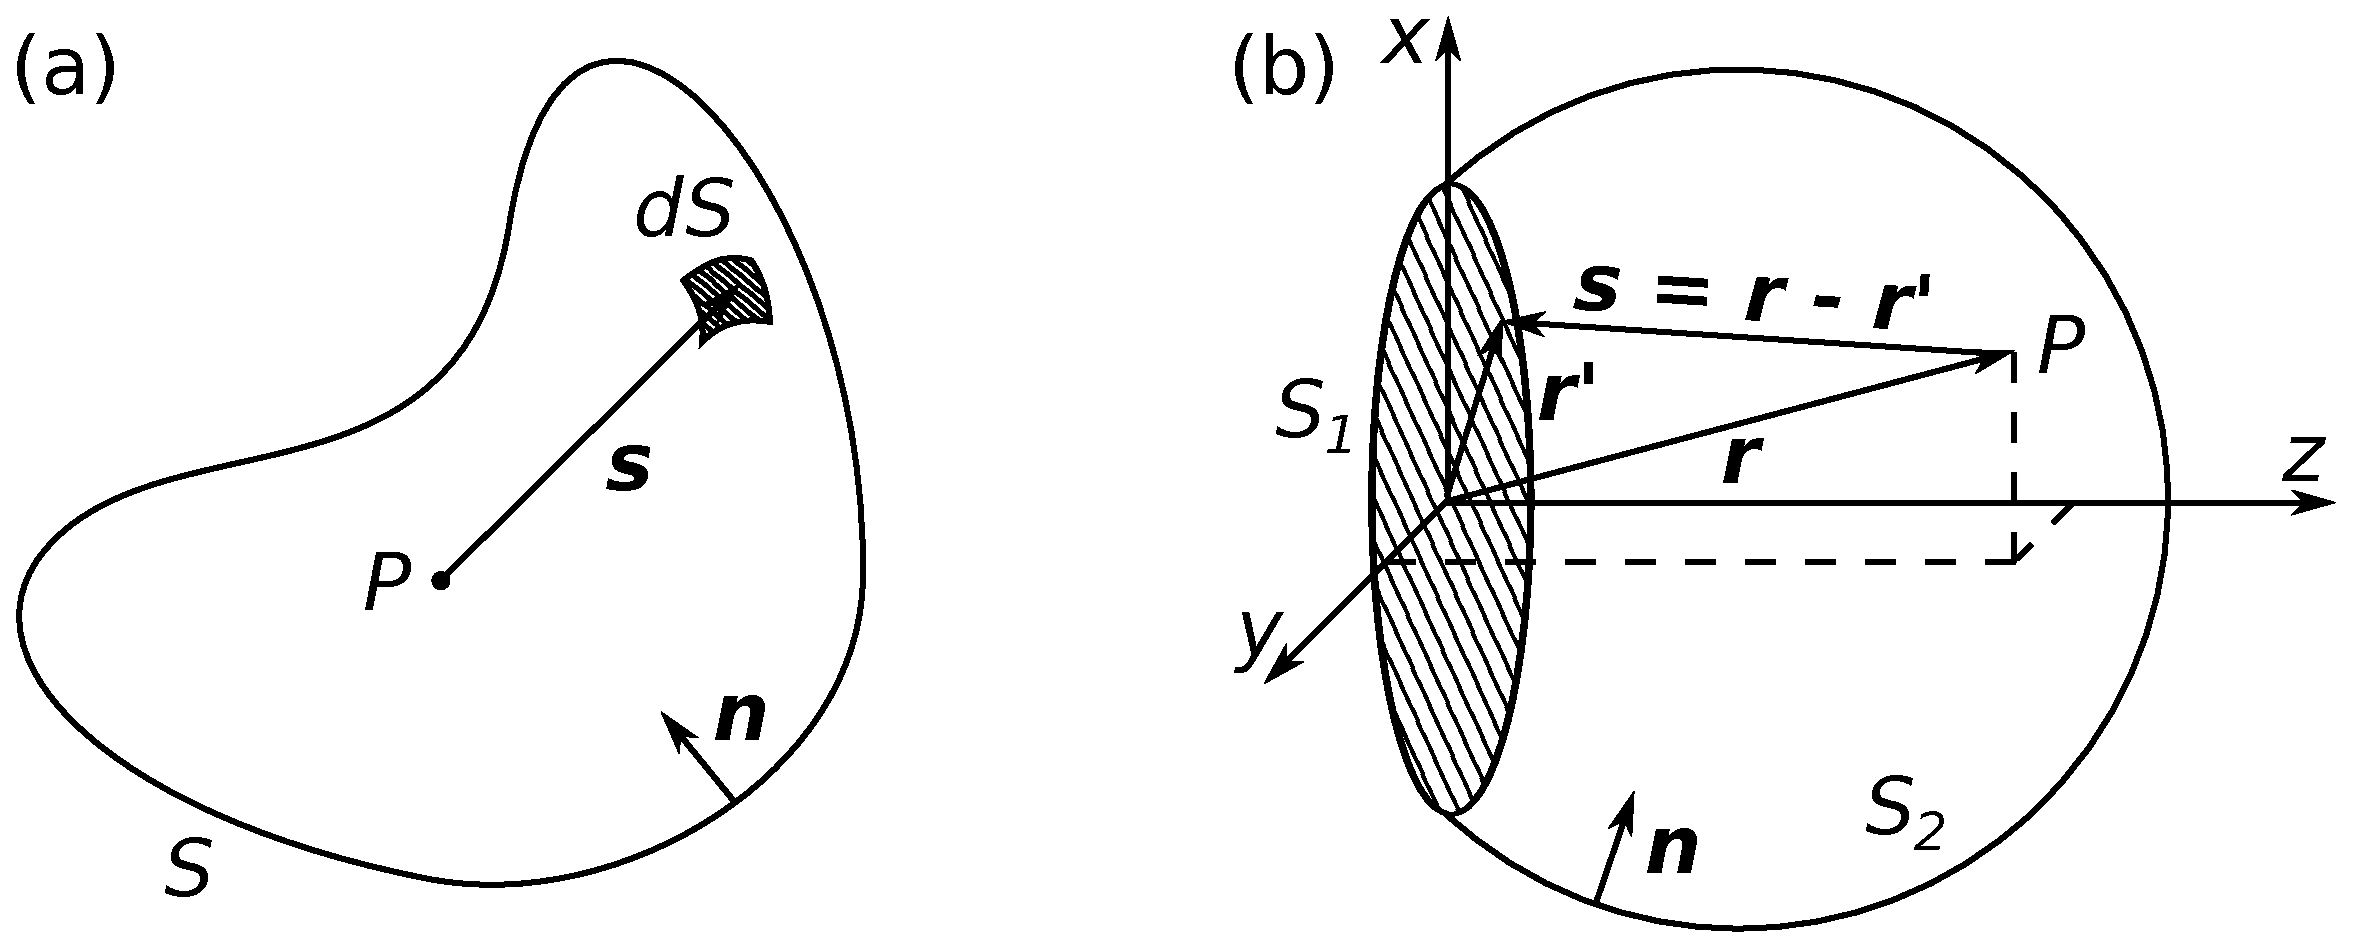
\includegraphics[width = \textwidth]{%
    Chapters/InterferometricMethods/figs/kirchhoff_geometry.eps}
  \caption[Geometries for Kirchhoff diffraction calculations]{%
    Geometries for Kirchhoff diffraction calculations.
    When $S_1$ is imaged by an optical system,
    $S_1$ is referred to as the \emph{object plane}.}
\label{fig:InterferometricMethods:Kirchhoff_geometry}
\end{figure}

To proceed with the diffraction calculation,
assume that the incident waves propagate in the $+z$-direction and
adopt the surface drawn
in Fig.~\ref{fig:InterferometricMethods:Kirchhoff_geometry}(b).
That is, $S = S_1 + S_2$,
where $S_1$ is a circle in the $(x, y)$-plane, and
$S_2$ is a spherical segment centered on the optical axis.
When $S_1$ is imaged by an optical system,
$S_1$ is referred to as the \emph{object plane}.
Now, assume that the incident waves were ``turned on''
at some finite time in the past, and
take the radius of $S_2$ to be large enough such that
none of the diffracted waves have had sufficient time to reach $S_2$,
i.e.\ $U \equiv 0$ on $S_2$.
(Of course, strictly speaking, the source's finite turn-on time
requires relaxation of the monochromatic assumption.
Finite turn-on time does not preclude a pseudo-monochromatic source, however,
and such a source is assumed hereafter).
Thus, the integral over $S_2$ vanishes, and
(\ref{eq:InterferometricMethods:Helmholtz_Kirchhoff_integral_theorem})
reduces to an integral over $S_1$.

Evaluation of
(\ref{eq:InterferometricMethods:Helmholtz_Kirchhoff_integral_theorem})
requires knowledge of $U$ on $S_1$.
For free-space propagation,
$S_1$ is an imagined (rather than a physical) surface
that does not impede the propagation of the incident beam $U^{(i)}$
(that is, $U = U^{(i)}$ and
$\partial U / \partial n = \partial U^{(i)} / \partial n$ on $S_1$).
If, however, $S_1$ contains opaque obstacles,
the free-space propagation conditions are no longer valid;
instead, the Kirchhoff boundary conditions can be adopted:
\begin{align}
  \text{surfaces of clear aperture:}&
  \quad
  U = U^{(i)},
  \quad
  \frac{\partial U}{\partial n} = \frac{\partial U^{(i)}}{\partial n}
  \\
  \text{opaque surfaces:}&
  \quad \;
  U = 0,
  \qquad
  \frac{\partial U}{\partial n} = 0
\end{align}
While these boundary conditions are adequate for the current application,
it should be noted that they are not physical
for points that are very close to the boundaries of the opaque obstacles.


\subsection{Fraunhofer diffraction of a free-space Gaussian beam}
Assume that the incident Gaussian beam has a waist at $S_1$, and
take the radius of $S_1$ to be much larger than the beam waist $w_0$
such that the domain of integration effectively extends
over the whole $(x, y)$-plane.
For free-space propagation,
$S_1$ does not perturb the Gaussian beam; thus,
$E(\vect{r}, t) = E^{(i)}(\vect{r}, t) = E_G(\vect{r}) e^{-i \omega_0 t}$.
Now, in the far-field ($k_0 s \gg 1$) and
paraxial ($\vect{s} \approx -z \hat{\vect{z}}$) approximations
\begin{align}
  \left. \frac{e^{i k_0 s}}{s} \right|_{S_1}
  &\approx
  \frac{e^{i k_0 s}}{z}
  \\
  \left. \frac{\partial}{\partial n}
  \left( \frac{e^{i k_0 s}}{s} \right) \right|_{S_1}
  &\approx
  -i k_0 \left( \frac{e^{i k_0 s}}{z} \right)
\end{align}
The $s$-dependence in the phase arguments has been retained,
as it is the mechanism responsible for diffraction, but
the $s$-dependence in the amplitude has been dropped
as it only gives rise to negligible variations
in the amplitude of the diffracted wave.
Relative to a spherical wave,
a Gaussian beam has several additional $z$-dependencies;
however, at the beam's waist
\begin{align}
  \left. \frac{\partial w(z)}{\partial z} \right|_{\text{waist}}
  &\equiv
  0
  \\
  \left. \frac{\partial}{\partial z}
  \left[ \frac{1}{R(z)} \right] \right|_{\text{waist}}
  &=
  \frac{1}{z_R^2}
  \\
  \left. \frac{\partial \psi(z)}{\partial z} \right|_{\text{waist}}
  &=
  \frac{1}{z_R}
\end{align}
Then, if the beam's Rayleigh range is much greater than
the probe wavelength ($k_0 z_R \gg 1$) and
the relevant transverse dimensions are much less than
the Rayleigh range ($w_0 \ll z_R$),
the Gaussian beam at $S_1$ satisfies
\begin{align}
  \left. E_G(\vect{r'}) \right|_{S_1}
  &\approx
  E_0 e^{-(\rho' / w_0)^2}
  \\
  \left. \frac{\partial E_G(\vect{r'})}{\partial n} \right|_{S_1}
  &\approx
  i k_0 \left[ E_0 e^{-(\rho' / w_0)^2} \right]
\end{align}
Note that the CO$_2$ laser beams ($k_0 \approx \SI{2 \pi e5}{\per\meter}$)
that probe tokamak plasmas often have $z_R \gg \SI{10}{\meter}$
such that $k_0 z_R \gg 1$ and $w_0 \ll z_R$
(the transverse dimensions are constrained by the machine size
such that $w_0 \ll \SI{1}{\meter}$) are very well satisfied.

Substituting the above expressions for
the incident waves and their surface-normal derivatives into
(\ref{eq:InterferometricMethods:Helmholtz_Kirchhoff_integral_theorem})
and simplifying yields
\begin{equation}
  E(\vect{r})
  \approx
  \frac{-i E_0}{\lambda_0 z}
  \int_{S_1}
  e^{-( \rho' / w_0 )^2}
  e^{i k_0 s}
  dS
  \label{eq:InterferometricMethods:Kirchhoff_diffraction_integral}
\end{equation}
To proceed further, $s$ must be approximated:
\begin{align}
  s
  &=
  | \vect{r'} - \vect{r}|
  \notag \\
  &=
  \left[ r^2 - 2(x'x + y'y) + (x'^2 + y'^2) \right]^{1/2}
  \notag \\
  &\approx
  r - \frac{x'x + y'y}{r}
  \label{eq:InterferometricMethods:Fraunhofer_s}
\end{align}
where only terms linear in $(x' / r)$ and $(y' / r)$ have been retained.
This is known as the Fraunhofer limit, and
it is valid for $z \gg z_R$~\cite[Sec.~8.3.3]{born_and_wolf}.
Under the Fraunhofer limit
(\ref{eq:InterferometricMethods:Kirchhoff_diffraction_integral}) becomes
\begin{equation}
  E(\vect{r})
  \approx
  \frac{-i E_0}{\lambda_0 z}
  e^{i k_0 r}
  D_x D_y
  \label{eq:InterferometricMethods:Fraunhofer_diffracted_field}
\end{equation}
where
\begin{align}
  D_x
  &=
  \int_{-\infty}^{\infty}
  e^{-( x' / w_0 )^2}
  e^{-i k_0 x' x / r}
  dx'
  \label{eq:InterferometricMethods:Fraunhofer_diffraction_integral_free_space}
  \\
  &=
  \mathcal{F} \left[%
    e^{-( x' / w_0 )^2}
  \right](k_0 x / r)
  \\
  &=
  \sqrt{\pi} w_0 e^{-(k_0 w_0 x / 2 r)^2}
  \label{eq:InterferometricMethods:Fourier_transform_free_space_Gaussian}
\end{align}
gives the diffraction pattern in the $x$-direction, and
the integral has been easily evaluated by noting that
it is simply the Fourier transform of a Gaussian.
The diffraction pattern in the $y$-direction, $D_y$, is similarly determined.
Note that the $e^{-i k_0 x' x / r} = e^{-i k_0 x' \sin\theta}$ term in
(\ref{eq:InterferometricMethods:Fraunhofer_diffraction_integral_free_space})
is the typical geometric phase factor
that results from path-length differences between
points on surface $S_1$ and the field point $\vect{r}$, as shown in
Fig.~{\ref{fig:InterferometricMethods:Fraunhofer_geometric_phase_factor}}.
Substituting
(\ref{eq:InterferometricMethods:Fourier_transform_free_space_Gaussian}) into
(\ref{eq:InterferometricMethods:Fraunhofer_diffracted_field}) yields
\begin{equation}
  E(\vect{r})
  \approx
  -i E_0
  \left( \frac{z_R}{z} \right)
  e^{-(k_0 w_0 \rho / 2 r)^2}
  e^{i k_0 r}
  \label{eq:InterferometricMethods:Fraunhofer_Gaussian_beam_diffraction}
\end{equation}
Is this consistent
with the expected far-field representation of a Gaussian beam? Yes!
To see this, note that in the far-field ($z \gg z_R$)
\begin{align}
  &\frac{z_R}{z}
  \approx
  \frac{w_0}{w(z)}
  \\
  &\frac{k_0 w_0 \rho}{2 r}
  \approx
  \frac{\rho}{w(z)}
  \\
  &r
  \approx
  z + \frac{\rho^2}{2 R(z)}
  \\
  &-i
  = e^{-i \pi / 2}
  \approx
  e^{-i \psi(z)}
\end{align}
such that
(\ref{eq:InterferometricMethods:Fraunhofer_Gaussian_beam_diffraction})
can be cast in the form of a typical Gaussian beam
as expressed in
(\ref{eq:InterferometricMethods:Gaussian_beam}),
i.e.\ $E(\vect{r}) = E_G(\vect{r})$ for $z \gg z_R$.
Of course, when considering free-space propagation,
$E(\vect{r}) \equiv E_G(\vect{r})$ for $0 \leq z < \infty$, but
the above work \emph{proves} that
the Fraunhofer diffraction formalism
gives the correct results under the appropriate limits;
it also lays the groundwork for examining
the diffraction of a phase-modulated Gaussian beam.

\begin{figure}
  \centering
  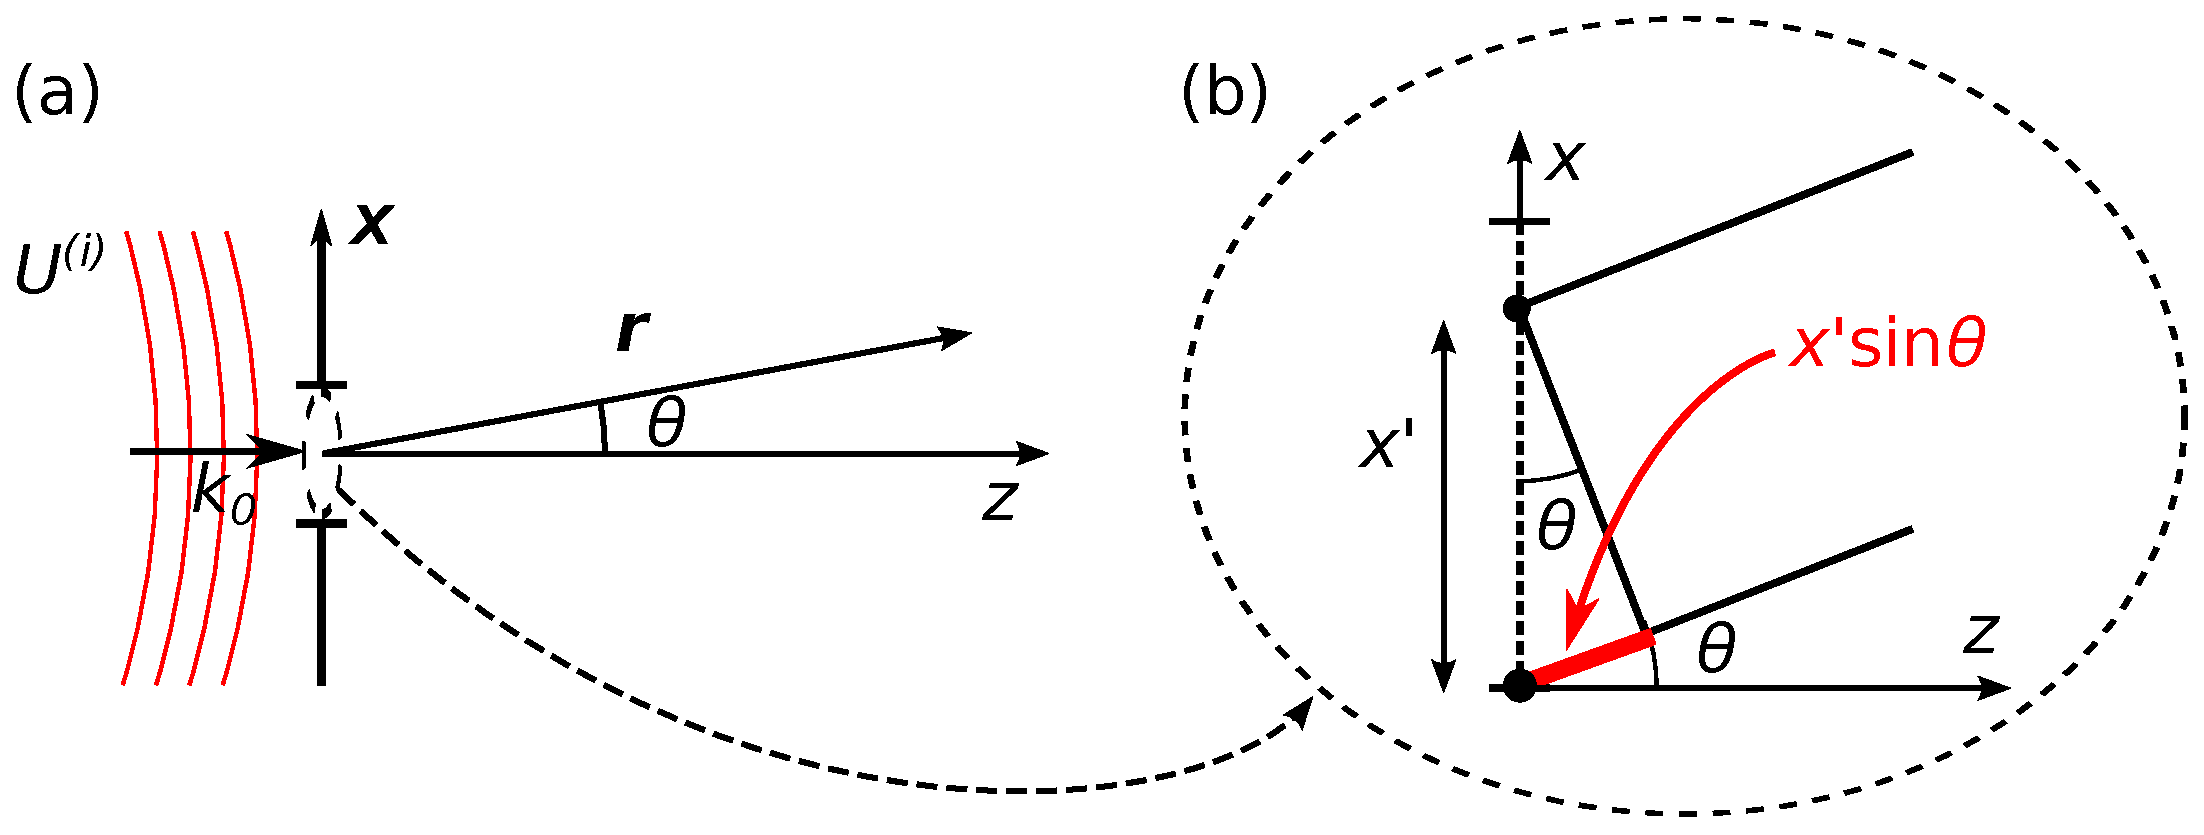
\includegraphics[width = \textwidth]{%
    Chapters/InterferometricMethods/figs/Fraunhofer_geometric_phase_factor.eps}
  \caption[Fraunhofer geometric phase factor]{%
    (a) Typical Fraunhofer diffraction geometry and
    (b) a close up that displays the path-length difference $x' \sin\theta$
    between a wave emanating from the origin and
    a wave emanating from $x'$}
\label{fig:InterferometricMethods:Fraunhofer_geometric_phase_factor}
\end{figure}


\subsection{Fraunhofer diffraction of a phase-modulated Gaussian beam}
Now, at $S_1$ allow the incident beam to see
an additional phase contribution $\phi$ that takes the form
\begin{equation}
  \phi(x', t) = \bar{\phi}(t) + \tilde{\phi}(x', t)
\end{equation}
Typically, $\tilde{\phi}$ varies on much faster time scales than $\bar{\phi}$
(quantitatively, $d(\ln \tilde{\phi})/dt \gg d(\ln \bar{\phi})/dt$), but
this is not required.
The response functions of the diagnostics investigated in
Sections~\ref{sec:InterferometricMethods:interferometry} and
\ref{sec:InterferometricMethods:pci} will be shown to be linear, so
it is sufficient to examine phase fluctuations $\tilde{\phi}$
consisting of a single Fourier mode
\begin{equation}
  \tilde{\phi}(x', t) = \tilde{\phi}_0 \cos(k x' - \omega t)
\end{equation}
This additional phase contribution modifies
(\ref{eq:InterferometricMethods:Fraunhofer_diffraction_integral_free_space})
such that the diffraction pattern in the $x$-direction is given as
\begin{align}
  D_x
  &=
  \int_{-\infty}^{\infty}
  e^{-( x' / w_0 )^2}
  e^{-i k_0 x x' / r}
  e^{i \phi(x', t)}
  dx'
  \notag \\
  &=
  e^{i \bar{\phi}}
  \int_{-\infty}^{\infty}
  e^{-( x' / w_0 )^2}
  e^{-i k_0 x x' / r}
  e^{i \tilde{\phi}_0 \cos(k x' - \omega t)}
  dx'
  \notag \\
  &=
  e^{i \bar{\phi}}
  \int_{-\infty}^{\infty}
  e^{-( x' / w_0 )^2}
  e^{-i k_0 x x' / r}
  \left\{%
    \sum_{m = -\infty}^{\infty}
    i^m \left[ J_m(\tilde{\phi}_0) \right]
    e^{i m (k x' - \omega t)}
  \right\}
  dx'
  \notag \\
  &=
  e^{i \bar{\phi}}
  \sum_{m = -\infty}^{\infty}
  i^m \left[ J_m(\tilde{\phi}_0) \right]
  e^{-i m \omega t}
  \int_{-\infty}^{\infty}
  e^{-( x' / w_0 )^2}
  e^{-i \left( \frac{k_0 x}{r} - m k \right) x'}
  dx'
  \notag \\
  &=
  \sqrt{\pi} w_0
  e^{i \bar{\phi}}
  \sum_{m = -\infty}^{\infty}
  i^m \left[ J_m(\tilde{\phi}_0) \right]
  e^{-i m \omega t}
  e^{-\left[ \frac{w_0}{2} \left( \frac{k_0 x}{r} - m k \right) \right]^2}
  \label{eq:InterferometricMethods:Fraunhofer_diffraction_integral_phase_modulated}
\end{align}
where the expression in the third line follows from
application of the well-known Jacobi-Anger expansion, and
$J_m$ is the $m$\ts{th} Bessel function of the first kind.
Noting that $E(\vect{r}, t) = E(\vect{r}) e^{-i \omega_0 t}$,
substitution of
(\ref{eq:InterferometricMethods:Fraunhofer_diffraction_integral_phase_modulated})
into (\ref{eq:InterferometricMethods:Fraunhofer_diffracted_field}) yields
\begin{align}
  \begin{aligned}
    E(\vect{r}, t)
    \approx
    e^{i \bar{\phi}}
    &\sum_{m = -\infty}^{\infty}
    i^m \left[ J_m(\tilde{\phi}_0) \right]
    e^{-i m \omega t}
    e^{-\left[ \frac{w_0}{2} \left( \frac{k_0 x}{r} - m k \right) \right]^2}
    \\
    &\times
    \left[
      -i E_0
      \left( \frac{z_R}{z} \right)
      e^{-(k_0 w_0 y / 2 r)^2}
      e^{i (k_0 r - \omega_0 t)}
    \right]
  \label{eq:InterferometricMethods:Fraunhofer_phase_modulated_Gaussian_beam_diffraction}
  \end{aligned}
\end{align}

\begin{figure}
  \centering
  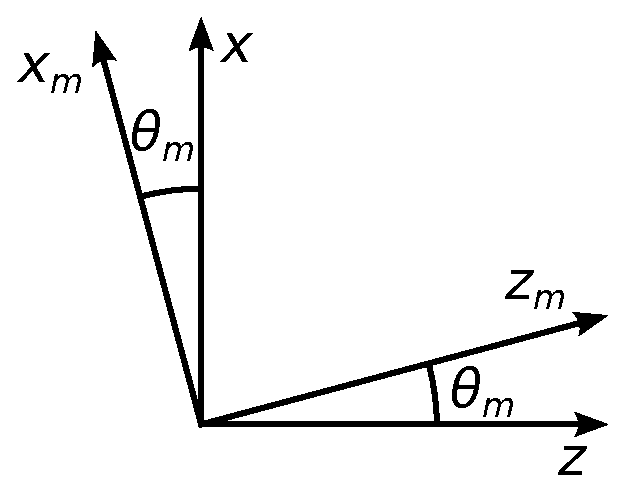
\includegraphics[width = 0.4 \textwidth]{%
    Chapters/InterferometricMethods/figs/coordinate_rotation.eps}
  \caption{Coordinate transformation for interpretation of
    the diffraction pattern of a phase-modulated Gaussian beam}
\label{fig:InterferometricMethods:coordinate_rotation}
\end{figure}

To put
(\ref{eq:InterferometricMethods:Fraunhofer_phase_modulated_Gaussian_beam_diffraction})
in a more familiar form,
consider the coordinate transformation
from the lab-frame coordinate system $\vect{r}$
to the coordinate system of the $m$\ts{th} scattered beam $\vect{r_m}$,
as depicted graphically
in Fig.~\ref{fig:InterferometricMethods:coordinate_rotation}.
As the transformation is simply
a rotation about the $y$-axis by angle $\theta_m$,
the coordinate systems are related via
\begin{equation}
  \begin{pmatrix}
    x_m
    \\
    y_m
    \\
    z_m
  \end{pmatrix}
  =
  \begin{pmatrix}
    \cos\theta_m & 0 & -\sin\theta_m
    \\
    0            & 1 & 0
    \\
    \sin\theta_m & 0 & \cos\theta_m
  \end{pmatrix}
  \begin{pmatrix}
    x
    \\
    y
    \\
    z
  \end{pmatrix}
  \label{eq:InterferometricMethods:object_plane_coordinate_transformation_explicit}
\end{equation}
where
\begin{equation}
  \sin \theta_m
  \equiv
  \frac{m k}{k_0}
  \label{eq:InterferometricMethods:scattering_angles}
\end{equation}
This coordinate transformation can be written more compactly as
\begin{equation}
  \vect{r_m}
  =
  \vect{R_m} \vect{r}
  \label{eq:InterferometricMethods:object_plane_coordinate_transformation_compact}
\end{equation}
where $\vect{R_m}$ is the rotation matrix in
(\ref{eq:InterferometricMethods:object_plane_coordinate_transformation_explicit}).
Rotation matrices are \emph{orthogonal},
which endows $\vect{R_m}$ with some useful properties
\cite[Ch.~6]{FB_linear_algebra};
namely, its inverse is equal to its transpose $\vect{R_m}^T$
\begin{equation}
  \vect{R_m}^T
  =
  \vect{R_m}^{-1}
  =
  \vect{R_{-m}}
  \label{eq:InterferometricMethods:rotation_matrix_inverse_relationships}
\end{equation}
and its determinant is unity
\begin{equation}
  \text{det}(\vect{R_m}) = |\vect{R_m}| = 1
  \label{eq:InterferometricMethods:rotation_matrix_determinant}
\end{equation}
such that the rotation preserves lengths, i.e.\ $r_m = r$.
Typically, $k / k_0 \ll 1$ such that the coordinate transforms reduce to
\begin{equation}
  \vect{r_m}
  =
  \begin{pmatrix}
    x_m
    \\
    y_m
    \\
    z_m
  \end{pmatrix}
  \approx
  \begin{pmatrix}
    x - z \theta_m
    \\
    y
    \\
    z + x \theta_m
  \end{pmatrix}
  \label{eq:InterferometricMethods:object_plane_coordinate_transformation_explicit_small_angle}
\end{equation}
and
\begin{equation}
  \vect{r}
  =
  \begin{pmatrix}
    x
    \\
    y
    \\
    z
  \end{pmatrix}
  \approx
  \begin{pmatrix}
    x_m + z_m \theta_m
    \\
    y_m
    \\
    z_m - x_m \theta_m
  \end{pmatrix}
  \label{eq:InterferometricMethods:object_plane_coordinate_transformation_explicit_small_angle_inverse}
\end{equation}
Substituting
(\ref{eq:InterferometricMethods:object_plane_coordinate_transformation_explicit_small_angle_inverse})
into
(\ref{eq:InterferometricMethods:Fraunhofer_phase_modulated_Gaussian_beam_diffraction})
and defining $\rho_m = (x_m^2 + y_m^2)^{1/2}$ yields
\begin{equation}
  \begin{aligned}
    E(\vect{r}, t)
    \approx
    e^{i \bar{\phi}}
    &\sum_{m = -\infty}^{\infty}
    i^m \left[ J_m(\tilde{\phi}_0) \right]
    e^{-i (\omega_0 + m \omega) t}
    \\
    &\times
    \left[
      -i E_0
      \left( \frac{z_R}{z_m} \right)
      e^{-(k_0 w_0 \rho_m / 2 r)^2}
      e^{i k_0 r}
    \right]
  \end{aligned}
\end{equation}
where the far-field limit has been used to approximate $1/z \approx 1/z_m$.
Now, the bracketed expression has the form of
(\ref{eq:InterferometricMethods:Fraunhofer_Gaussian_beam_diffraction})
for a far-field Gaussian beam; thus,
the diffracted electric field can be more compactly and generally written as
\begin{equation}
  E(\vect{r}, t)
  \approx
  e^{i \bar{\phi}}
  \sum_{m = -\infty}^{\infty}
  i^m \left[ J_m(\tilde{\phi}_0) \right]
  E_G(\vect{r_m})
  e^{-i (\omega_0 + m \omega) t}
  \label{eq:InterferometricMethods:phase_modulated_Gaussian_beam_diffraction}
\end{equation}
Note that
(\ref{eq:InterferometricMethods:phase_modulated_Gaussian_beam_diffraction})
is valid for $0 \leq z < \infty$ rather than only for $z \gg z_R$;
that is, computing the far-field diffraction pattern
has additionally allowed inferring the corresponding near-field.

Thus, a sinusoidal phase modulation diffracts an incident Gaussian beam
into an infinite number of \emph{scattered} Gaussian beams.
The incident beam is coupled into the $m$\ts{th} scattered beam
with strength $J_m(\tilde{\phi}_0)$.
The $m$\ts{th} scattered beam is Doppler shifted
relative to the incident beam by $m \omega$ and
propagates at an angle $\theta_m \approx m k / k_0$
relative to the lab-frame optical axis.
Note that the spatial dependence of the scattered beams' phase evolution
remains $e^{i [k_0 r - \psi(z)]}$; that is,
the scattering process is elastic,
with $|\vect{k^{(i)}}| = |\vect{k_m}| = k_0$.
This constraint of elasticity
coupled with knowledge of the scattering angle $\theta_m$
allows determination of the scattered wavevector
\begin{equation}
  \vect{k_m}
  =
  (m k) \hat{\vect{x}}
  +
  k_0 \left[ 1 - \left(\frac{m k}{k_0}\right)^2 \right]^{1/2} \hat{\vect{z}}
  %k_0 \sqrt{1 - \left(\frac{m k}{k_0}\right)^2} \hat{\vect{z}}
  \label{eq:InterferometricMethods:scattered_beam_wavevector}
\end{equation}

Obviously, the scalar nature of the above diffraction calculation
is insufficient to capture
the small polarization changes that accompany beam scattering.
Such polarization changes are of little interest in this work, so
their theoretical treatment is not pursued here.


\subsection{Wavenumber-dependent manipulation of diffracted Gaussian beams}
Examine again
(\ref{eq:InterferometricMethods:phase_modulated_Gaussian_beam_diffraction}).
Note that the spatial dependence of the diffracted field
is governed entirely by the factor $E_G(\vect{r_m})$,
which specifies the spatial structure of the $m$\ts{th} diffracted beam.
Note that $E_G(\vect{r_m})$ can be Fourier decomposed as
\begin{align}
  E_G(\vect{r_m})
  &=
  \mathcal{F}^{-1}[E_G(\vect{k_m}')](\vect{r_m})
  \notag \\
  &=
  \frac{1}{(2 \pi)^3}
  \int d\vect{k_m}'
  e^{i \vect{k_m}' \cdot \vect{r_m}}
  E_G(\vect{k_m}')
  \notag \\
  &=
  \frac{1}{(2 \pi)^3}
  \int d\vect{k_m}'
  e^{i \vect{k_m}' \cdot \vect{r_m}}
  \left[
    \int d\vect{r}' \,
    e^{-i \vect{k_m}' \cdot \vect{r}'}
    E_G(\vect{r}')
  \right]
  \notag \\
  &=
  \frac{1}{(2 \pi)^3}
  \int d\vect{r}' \,
  E_G(\vect{r}')
  \int d\vect{k_m}' \,
  e^{i \vect{k_m}' \cdot (\vect{r_m} - \vect{r}')}
  \notag
\end{align}
where $\vect{k_m}'$ is the wavevector basis that is \emph{dual} to
the coordinate system of the $m$\ts{th} scattered beam, $\vect{r_m}$.
To understand the significance of this duality,
note that $\vect{k_m}' \cdot \vect{r_m}$ is a physical quantity,
independent of any given coordinate system; that is,
if $\vect{k}'$ is the wavevector basis dual to
the lab-frame (i.e. $m = 0$ beam) coordinate system, then, by definition,
$\vect{k_m}' \cdot \vect{r_m} = \vect{k}' \cdot \vect{r}$.
Enforcing this coordinate-independent requirement and
exploiting the orthogonality of $\vect{R_m}$ yields
\begin{align}
  \vect{k}' \cdot \vect{r}
  &=
  \vect{k}'^T \vect{r}
  \notag \\
  &=
  \vect{k}'^T (\vect{R_m}^T \vect{R_m}) \vect{r}
  \notag \\
  &=
  (\vect{R_m} \vect{k}')^T (\vect{R_m} \vect{r})
  \notag \\
  &=
  (\vect{R_m} \vect{k}') \cdot \vect{r_m}
  \notag \\
  &=
  \vect{k_m}' \cdot \vect{r_m}
  \notag
\end{align}
such that
\begin{equation}
  \vect{k_m}'
  =
  \vect{R_m} \vect{k}'
  \label{eq:InterferometricMethods:wavevector_dual_to_mth_beam}
\end{equation}

While the above Fourier decomposition is trivial,
it lays the foundation for more sophisticated analysis.
For example, imagine that the Fourier components of $E_G(\vect{r_m})$
are somehow manipulated
based upon lab-frame wavenumber $\vect{k}'$;
if this manipulation can be described
in terms of a transfer function $T(\vect{k}')$,
then the resulting spatial dependence
of the $m$\ts{th} diffracted beam is
\begin{align}
  \mathcal{E}_G(\vect{r_m})
  &=
  \frac{1}{(2 \pi)^3}
  \int d\vect{r}' \,
  E_G(\vect{r}')
  \int d\vect{k_m}' \,
  T(\vect{k}')
  e^{i \vect{k_m}' \cdot (\vect{r_m} - \vect{r}')}
\end{align}
where the notation $\mathcal{E}_G(\vect{r_m})$
has been selected to emphasize that
this spatial dependence may differ from $E_G(\vect{r_m})$.
Note that the wavevector integration variables are
with respect to the basis of the $m$\ts{th} scattered beam $\vect{k_m}'$
whereas the transfer function is expressed in terms of
the lab-frame basis $\vect{k}'$.
To proceed, change the variables of integration
from $\vect{k_m}'$ to $\vect{k}'$ by noting that
\begin{equation}
  d\vect{k_m}'
  =
  \left| \frac{\partial \vect{k_m}'}{\partial \vect{k}'} \right|
  d\vect{k}'
  =
  |\vect{R_m}|
  d\vect{k}'
  =
  d\vect{k}'
  \notag
\end{equation}
and
\begin{align}
  \vect{k_m}' \cdot (\vect{r_m} - \vect{r}')
  &=
  (\vect{R_m}\vect{k}') \cdot (\vect{R_m}\vect{r} - \vect{r}')
  \notag \\
  &=
  (\vect{R_m}\vect{k}')^T (\vect{R_m}\vect{r} - \vect{r}')
  \notag \\
  &=
  \vect{k}'^T \vect{R_m}^T (\vect{R_m}\vect{r} - \vect{r}')
  \notag \\
  &=
  \vect{k}'^T (\vect{R_m}^T\vect{R_m}\vect{r} - \vect{R_m}^T\vect{r}')
  \notag \\
  &=
  \vect{k}' \cdot \left[ \vect{r} - \left(\vect{R_{-m}}\vect{r}'\right) \right]
  \notag \\
  &=
  \vect{k}' \cdot \left( \vect{r} - \vect{r_{-m}}' \right)
  \notag
\end{align}
such that $\mathcal{E}_G(\vect{r_m})$ becomes
\begin{align}
  \mathcal{E}_G(\vect{r_m})
  &=
  \frac{1}{(2 \pi)^3}
  \int d\vect{r}' \,
  E_G(\vect{r}')
  \int d\vect{k}' \,
  T(\vect{k}')
  e^{i \vect{k}' \cdot (\vect{r} - \vect{r_{-m}}')}
  \label{eq:InterferometricMethods:mth_diffracted_beam_Fourier_filtered}
\end{align}

To make further progress,
a particular form of $T(\vect{k}')$ is needed.
Assume that $T(\vect{k}') = T(k_x')$ such that
wavenumbers are filtered only in the direction of beam scattering.
Then (\ref{eq:InterferometricMethods:mth_diffracted_beam_Fourier_filtered})
becomes
\begin{align}
  \mathcal{E}_G(\vect{r_m})
  &=
  \frac{1}{(2 \pi)^3}
  \int d\vect{r}' \,
  E_G(\vect{r}')
  \int dk_x' \,
  T(k_x')
  e^{i k_x' (x - x_{-m}')}
  \notag \\
  &\qquad\qquad \times
  \int dk_y' \,
  e^{i k_y' (y - y_{-m}')}
  \int dk_z' \,
  e^{i k_z' (z - z_{-m}')}
  \notag \\
  &=
  \frac{1}{2 \pi}
  \int d\vect{r}' \,
  E_G(\vect{r}')
  \delta(y - y_{-m}')
  \delta(z - z_{-m}')
  \notag \\
  &\qquad\qquad \times
  \int dk_x' \,
  T(k_x')
  e^{i k_x' (x - x_{-m}')}
  \notag \\
  &\begin{aligned}
    &=
    \frac{1}{2 \pi}
    \int dx' \,
    E_G(x', y, z + x' \theta_m)
    \\
    &\qquad\qquad \times
    \int dk_x' \,
    T(k_x')
    e^{i k_x' (x - x_{-m}')}
  \end{aligned}
  \notag \\
  &\begin{aligned}
    &=
    \frac{1}{2 \pi}
    \int dx' \,
    E_G(x', y, z + x' \theta_m)
    \\
    &\qquad\qquad \times
    \int dk_x' \,
    T(k_x')
    e^{i k_x' (x_m - x')}
  \end{aligned}
  \label{eq:InterferometricMethods:mth_diffracted_beam_kx_filtered_v1}
\end{align}
Contributions to the integral from regions outside of $|x'| \lesssim w(z)$
are suppressed by the Gaussian envelope such that
\begin{align}
  w(z + x' \theta_m)
  &\approx
  w(z)
  \notag \\
  R(z + x' \theta_m)
  &\approx
  R(z)
  \notag \\
  \psi(z + x' \theta_m)
  &\approx
  \psi(z)
  \notag
\end{align}
are very good approximations
when evaluating $E_G(x', y, z + x' \theta_m)$.
Note that the phase factor $\exp[i k_0 (z + x' \theta_m)]$
must be fully retained
(that is, $\exp[i k_0 (z + x' \theta_m)] \not\approx\exp[i k_0 z]$).
After making these approximations,
(\ref{eq:InterferometricMethods:mth_diffracted_beam_kx_filtered_v1})
reduces to
\begin{equation}
  \mathcal{E}_G(\vect{r_m})
  \approx
  E_G(0, y, z)
  \cdot
  \mathcal{P}(m, k, x)
  \label{eq:InterferometricMethods:mth_diffracted_beam_kx_filtered_compact}
\end{equation}
where
\begin{equation}
  \begin{aligned}
    \mathcal{P}(m, k, x)
    &=
    \frac{1}{2 \pi}
    \int dx' \,
    \exp\left[ \frac{-x'^2}{w(z)^2} \right]
    \exp\left\{%
      i \left[%
        m k x'
        +
        \frac{k_0 x'^2}{2 R(z)}
      \right]
    \right\}
    \\
    &\qquad \times
    \int dk_x' \,
    T(k_x')
    e^{i k_x' (x_m - x')}
  \end{aligned}
  \label{eq:InterferometricMethods:mth_diffracted_beam_kx_filtered_phase_factor}
\end{equation}
is a complex-valued phase factor
that results from filtering the scattered radiation by $T(k_x')$.
Generalizing
(\ref{eq:InterferometricMethods:phase_modulated_Gaussian_beam_diffraction})
to allow for such wavenumber-dependent manipulation
yields a total diffracted electric field
\begin{equation}
  E(\vect{r}, t)
  \approx
  e^{i \bar{\phi}}
  \sum_{m = -\infty}^{\infty}
  i^m \left[ J_m(\tilde{\phi}_0) \right]
  \mathcal{E}_G(\vect{r_m})
  e^{-i (\omega_0 + m \omega) t}
  \label{eq:InterferometricMethods:phase_modulated_Gaussian_beam_diffraction_Fourier_filtered}
\end{equation}
Manipulating the total diffracted electric field in such a manner
forms the foundation of phase contrast imaging (PCI),
as will be demonstrated in Section~\ref{sec:InterferometricMethods:pci}.


\section{Imaging of the diffracted beams}
It is often desirable to \emph{image} the above diffracted beams
in order to determine the spatiotemporal aspects
of the responsible phase fluctuations.
Below, the geometric optics and Gaussian beam propagation
of relevance to imaging systems is briefly reviewed
prior to computing the imaged field.


\subsection{The geometric optics of an imaging system}
Let the optical axis of an arbitrary optical system lie along the $z$-axis,
and let all optical rays lie in a plane with the optical axis.
At a given position $z_j$, an optical ray is fully described by
its transverse distance $\rho$ to the optical axis and
its slope $d\rho / dz$.
In the paraxial limit $d\rho / dz \approx \theta$
where $\theta$ is the angle between the ray and the optical axis.
Ray propagation through homogeneous media and refractive interfaces
are well-governed by the so-called $ABCD$ ray matrix formalism
\cite[Ch.~15]{siegman_lasers};
that is, a ray propagating from point $j$ to point $j + 1$ evolves as
\begin{equation}
  \begin{pmatrix}
    \rho_{j + 1}
    \\
    \theta_{j + 1}
  \end{pmatrix}
  =
  \begin{pmatrix}
    A & B
    \\
    C & D
  \end{pmatrix}
  \begin{pmatrix}
    \rho_j
    \\
    \theta_j
  \end{pmatrix}
  \label{eq:InterferometricMethods:ABCD_ray_tracing_general}
\end{equation}
where the $ABCD$ matrix elements are determined
by the optical properties of the media between points $j$ and $j + 1$.

An imaging system $\image$, by definition,
redirects all rays emanating from transverse position $\rho_{\object}$
in the object plane $S_{\object}$
to intersect at transverse position
$\rho_{\image} = M \rho_{\object}$
in the image plane $S_{\image}$.
Here, $M$ is the \emph{magnification} of the imaging system, and
$M < 0$ implies that the image is inverted relative to the object.
The imaging system's $A$, $B$, and $D$ matrix elements
are easily determined by inspection.
Recalling the definition in
(\ref{eq:InterferometricMethods:ABCD_ray_tracing_general}),
note that
$\rho_{\image} = M \rho_{\object} = A \rho_{\object} + B \theta_{\object}$
such that $A = M$ and $B = 0$.
Further, assuming the image plane and object plane refractive indices
are identical, as is often the case,
the determinant of the ray matrix is unity
(i.e.\ $AD - BC = 1$)~\cite{halbach_63}
such that $D = 1 / M$.
The final matrix element $C$ is determined by the particulars
of the imaging system;
for propagation through ``simple'' optical components,
such as lenses and homogeneous media, $C$ is constrained to be real.
Thus, an imaging system of magnification $M$ is characterized
by a ray matrix of the form
\begin{equation}
  \mathcal{I}
  =
  \begin{pmatrix}
    M & 0
    \\
    C & 1 / M
  \end{pmatrix}
  \label{eq:InterferometricMethods:ABCD_imaging}
\end{equation}

Now, the optical axis of each diffracted Gaussian beam
behaves as a ray in the geometric-optics sense
\cite{tovar_generalized_beam_matrices_IV}.
Thus, the $m$\ts{th} diffracted beam is rotated by angle $\theta_m / M$
relative to the undiffracted beam in the imaging plane,
as shown in Fig.~\ref{fig:InterferometricMethods:imaging_geometry}.
Further, the phase-fluctuation wavevector $k$ is imaged as $k / M$ such that
the wavevector of the $m$\ts{th} diffracted beam in the image plane is
\begin{align}
  \vect{k_{m,\image}}
  =
  \left( \frac{m k}{M} \right) \hat{\vect{x}}
  +
  k_0 \left[ 1 - \left(\frac{m k}{M k_0}\right)^2 \right]^{1/2} \hat{\vect{z}}
  %k_0 \sqrt{1 - \left(\frac{m k}{k_0}\right)^2} \hat{\vect{z}}
  \label{eq:InterferometricMethods:scattered_beam_wavevector_image_plane}
\end{align}
Note that
(\ref{eq:InterferometricMethods:scattered_beam_wavevector_image_plane})
is consistent with the $m$\ts{th} diffracted beam having an angle
$\theta_m / M$ relative to the optical axis in the image plane.

\begin{figure}
  \centering
  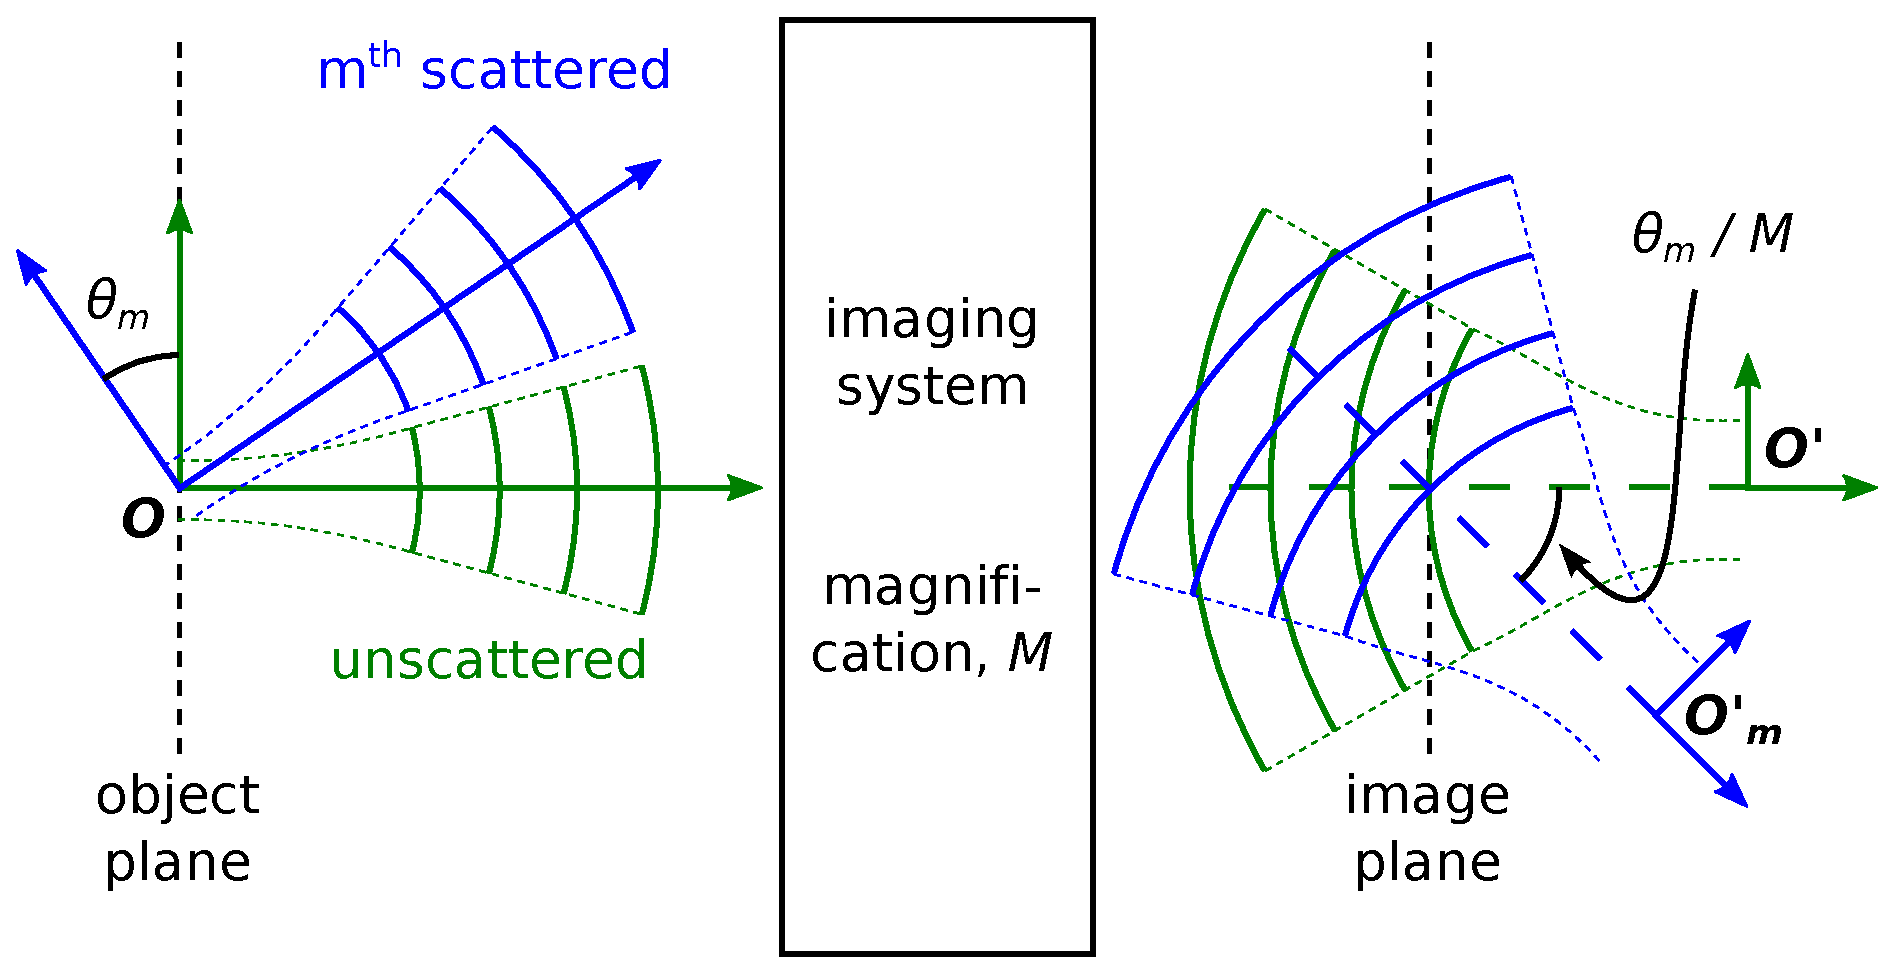
\includegraphics[width = \textwidth]{%
    Chapters/InterferometricMethods/figs/imaging_geometry.eps}
  \caption[Imaging geometry]{%
    Beam geometries in an imaging system with magnification $M$.
    Beam scattering occurs in the object plane at the probe beam's waist.
    Thus, the $m$\ts{th} scattered beam
    shares the origin $\vect{O}_{\object}$ with the unscattered beam but
    is angularly separated by $\theta_m$.
    The imaging system redirects all beams emanating from $\vect{O}_{\object}$
    to intersect at angle $\theta_m / M$ in the image plane.
    In general, the image plane does \emph{not} sit at a beam waist
    such that the post-imaging-system beam waists
    of the scattered and unscattered beams do not coincide,
    i.e.\ $\vect{O}_{\image} \neq \vect{O}_{m,\image}$.}
\label{fig:InterferometricMethods:imaging_geometry}
\end{figure}


\subsection{Gaussian beam transformation in an imaging system}
\label{sec:InterferometricMethods:imaging:Gaussian_beam_transformation}
In addition to manipulating the ray-like trajectory
of a Gaussian beam's optical axis,
an imaging system also alters
other important properties of an incident Gaussian beam.
A Gaussian beam is fully characterized by
its in-medium wavelength $\lambda_0 / N$,
its width $w(z_j)$, and
its radius of curvature $R(z_j)$
at a single location $z_j$.
These parameters can be conveniently combined
to define the so-called complex beam parameter $q$
\cite[Sec.~17.1]{siegman_lasers}
\begin{equation}
  \frac{1}{q}
  \equiv
  \frac{1}{R}
  -
  i \left( \frac{\lambda_0}{N \pi w^2} \right)
  \label{eq:InterferometricMethods:complex_beam_parameter_inverse}
\end{equation}
Referencing (\ref{eq:InterferometricMethods:Gaussian_beam_width}) and
(\ref{eq:InterferometricMethods:Gaussian_beam_radius_of_curvature}),
the complex beam parameter can be rewritten as
\begin{equation}
  q = z + i z_R
  \label{eq:InterferometricMethods:complex_beam_parameter}
\end{equation}
where, again, $z$ is the axial distance from the beam waist.
The Gaussian beam can then be propagated from point $j$ to point $j + 1$ via
\begin{equation}
  q_{j+1}
  =
  \frac{A q_j + B}{C q_j + D}
  \label{eq:InterferometricMethods:complex_beam_parameter_propagation}
\end{equation}
where, amazingly, $A$, $B$, $C$, and $D$
are equal to the corresponding values
of the $ABCD$ ray matrix from geometric optics
\cite[Sec.~20.2]{siegman_lasers}.
Using the ray matrix of an imaging system from
(\ref{eq:InterferometricMethods:ABCD_imaging}),
the image-plane complex beam parameter $q_{\image}$ is given as
\begin{equation}
  q_{\image}
  =
  \frac{M q_{\object}}{C q_{\object} + (1 / M)}
  \label{eq:InterferometricMethods:complex_beam_parameter_image_plane}
\end{equation}
where $q_{\object}$ is the object-plane complex beam parameter,
and $M$ and $C$ are both real.

To determine the imaged field,
both the undiffracted and the diffracted beams
must be propagated through the imaging system.
Fortunately, for a given optical system in the paraxial limit,
a Gaussian beam's width and radius of curvature evolve independently of
its transverse and angular displacements from
the nominal optical axis
\cite{tovar_generalized_beam_matrices_IV}.
That is, as any given diffracted beam
propagates through an imaging system $\image$,
the evolution of its width and radius of curvature
will be \emph{identical} to that of the undiffracted beam
propagating through the same imaging system.
However, the post-imaging-system beam waists
do \emph{not} necessarily sit at the image plane,
in which case the beams' native coordinate systems
are necessarily displaced from each other
(i.e.\ $\vect{O}_{\image} \neq \vect{O}_{m,\image}$),
as indicated in Fig.~\ref{fig:InterferometricMethods:imaging_geometry}.
Examining (\ref{eq:InterferometricMethods:complex_beam_parameter_image_plane})
it is easy to see that the beam waists will not sit at the image plane
when $C q_{\object} \gg 1 / M$ such that
$z_{\image} = \text{Re}(q_{\image}) \approx M / C \neq 0$.

As the native coordinate systems of
the undiffracted beam and the $m$\ts{th} diffracted beam
do not align in the image plane,
it will be convenient to determine the relevant coordinate transformation.
The transformation is derived for the most general case
in which the beam waists do not sit at the image plane
(i.e.\ $\vect{O}_{\image} \neq \vect{O}_{m,\image}$).
The coordinate transformation is easily found
through a series of translations and rotations, but
it may be useful to refer to
Fig.~\ref{fig:InterferometricMethods:coordinate_transformation_imaging_plane}
in the following discussion.
Let point $P$ be represented
in the native coordinate system of the unscattered beam
\graffito{\textcolor{red}{need to correct notation here}}
by the ordered pair $(z_0', x_0')$.
Then, the representation of $P$ in the $\alpha$-base is
\begin{equation}
  \begin{pmatrix}
    z_{\alpha}' \\
    x_{\alpha}'
  \end{pmatrix}
  =
  \begin{pmatrix}
    z_0' - z' \\
    x_0'
  \end{pmatrix}
\end{equation}
The $\alpha$- and $\beta$-bases are related via a rotation
\begin{equation}
  \begin{pmatrix}
    z_{\beta}' \\
    x_{\beta}'
  \end{pmatrix}
  =
  \begin{pmatrix}
    \cos\left( \frac{\theta_m}{M} \right)
    &
    \sin\left( \frac{\theta_m}{M} \right)
    \\
    -\sin\left( \frac{\theta_m}{M} \right)
    &
    \cos\left( \frac{\theta_m}{M} \right)
  \end{pmatrix}
  \begin{pmatrix}
    z_{\alpha}' \\
    x_{\alpha}'
  \end{pmatrix}
\end{equation}
Finally, a linear translation converts the $\beta$-base
into the native coordinate system of the $m$\ts{th} scattered beam
in the image plane
\begin{equation}
  \begin{pmatrix}
    z_m' \\
    x_m'
  \end{pmatrix}
  =
  \begin{pmatrix}
    z_{\beta}' +  z' \\
    x_{\beta}'
  \end{pmatrix}
\end{equation}
Combining the above steps and
evaluating at the image plane ($z_0' = z', \, x_0' = x'$)
yields the image-plane coordinate transformation
\begin{equation}
  \begin{pmatrix}
    z_m' \\
    x_m'
  \end{pmatrix}
  =
  \begin{pmatrix}
    z' + x' \sin\left( \frac{\theta_m}{M} \right) \\
    x' \cos\left( \frac{\theta_m}{M} \right)
  \end{pmatrix}
  \approx
  \begin{pmatrix}
    z' + \left( \frac{m k}{M k_0} \right) x' \\
    x' - \frac{1}{2} \left( \frac{m k}{M k_0} \right)^2 x'
  \end{pmatrix}
  \label{eq:InterferometricMethods:coordinate_transformation_imaging_plane}
\end{equation}
where the approximation holds for
the typical small-angle scattering limit ($\theta_m \ll 1$).

\begin{figure}
  \centering
  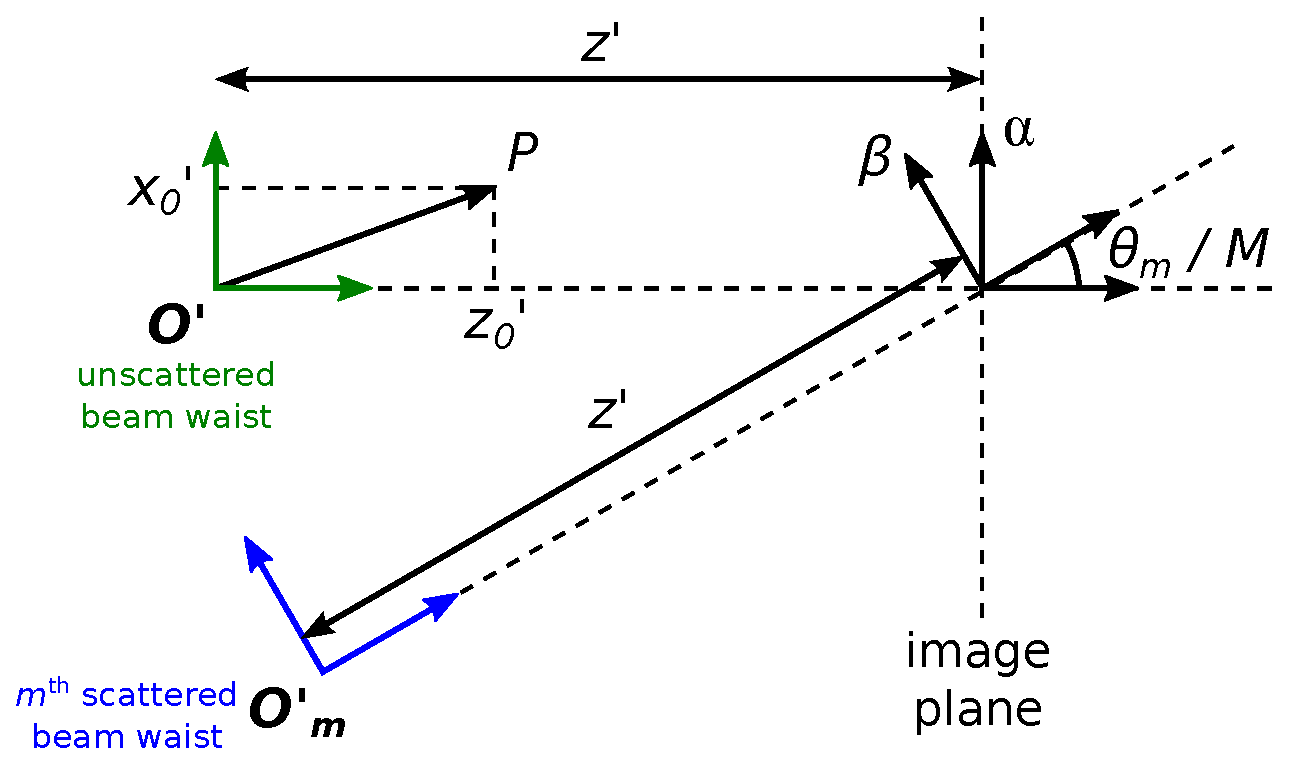
\includegraphics[width = 0.9 \textwidth]{%
    Chapters/InterferometricMethods/figs/coordinate_transformation_imaging_plane.eps}
  \caption[Image-plane coordinate transformation]{%
    Image-plane coordinate transformation}
\label{fig:InterferometricMethods:coordinate_transformation_imaging_plane}
\end{figure}


\subsection{The imaged field}
Now, without further ado,
let $\image$ image the object plane $S_{\object}$
such that the image of diffracted field
(\ref{eq:InterferometricMethods:phase_modulated_Gaussian_beam_diffraction_Fourier_filtered})
is
\begin{align}
  E(\vect{r}_{\image}, t)
  &=
  \image[ E(\vect{r}_{\object}, t) ]
  \notag \\
  &=
  e^{i \bar{\phi}}
  \sum_{m = -\infty}^{\infty}
  i^m \left[ J_m(\tilde{\phi}_0) \right]
  \image[\mathcal{E}_G(\vect{r}_{m,\object})]
  e^{-i (\omega_0 + m \omega) t}
  \label{eq:InterferometricMethods:imaged_total_field_v1}
\end{align}
where the linearity of $\image$ has been invoked
to bring the operator within the summation.
Referencing
(\ref{eq:InterferometricMethods:mth_diffracted_beam_kx_filtered_compact}),
it readily follows that
\begin{align}
  \image[\mathcal{E}_G(\vect{r}_{m,\object})]
  &=
  \mathcal{I}[%
    E_G(0, y_{\object}, z_{\object})
    \cdot
    \mathcal{P}(m, k, x_{\object})
  ]
  \notag \\
  &=
  E_G(0, y_{\image}, z_{\image})
  \cdot
  \mathcal{P}(m, k_{\image}, x_{\image})
\end{align}
where the object-plane wavevector $k$ has been imaged as
\begin{equation}
  k_{\image} = \frac{k}{M}
\end{equation}
Thus, (\ref{eq:InterferometricMethods:imaged_total_field_v1}) becomes
\begin{equation}
  \begin{aligned}
    E(\vect{r}_{\image}, t)
    &=
    E_G(0, y_{\image}, z_{\image}, t)
    e^{i \bar{\phi}}
    \\
    &\quad \times
    \sum_{m = -\infty}^{\infty}
    i^m \left[ J_m(\tilde{\phi}_0) \right]
    \mathcal{P}(m, k_{\image}, x_{\image})
    e^{-i m \omega t}
  \end{aligned}
  \label{eq:InterferometricMethods:imaged_total_field}
\end{equation}
where
$E_G(0, y_{\image}, z_{\image}, t)
=
E_G(0, y_{\image}, z_{\image}) e^{-i \omega_0 t}$.


\subsection{The weak-coupling limit}
Typically, the phase-fluctuation amplitude
is very small ($\tilde{\phi}_0 \ll 1$), and
the Bessel function's small-argument limiting form \cite{abramowitz_and_stegun}
can be used
\begin{equation}
  \lim_{z \rightarrow 0} J_m(z)
  \sim
  \begin{cases}
    \frac{1}{\Gamma(m + 1)} \left( \frac{z}{2} \right)^m
    , \qquad
    &m = 0, 1, 2, 3, \cdots
    \\
    \frac{1}{\Gamma(|m| + 1)} \left( \frac{-z}{2} \right)^{|m|}
    , \qquad
    &m = -1, -2, -3, \cdots
  \end{cases}
\end{equation}
Here, $\Gamma$ is the gamma function, and
$\Gamma(m + 1) = m!$ for positive integer $m$.
Dropping terms exceeding first order in $\tilde{\phi}_0$ and
introducing the notational shorthand
$\mathcal{P}_m \equiv \mathcal{P}(m, k_{\image}, x_{\image})$,
(\ref{eq:InterferometricMethods:imaged_total_field}) becomes
\begin{equation}
  \begin{aligned}
  E(\vect{r}_{\image}, t)
  &\approx
  E_G(0, y_{\image}, z_{\image}, t)
  e^{i \bar{\phi}}
  \\
  &\quad\times
  \biggl\{%
    \mathcal{P}_{0}
    +
    i \frac{\tilde{\phi}_0}{2}
    \left[
      \mathcal{P}_{1} e^{-i \omega t}
      +
      \mathcal{P}_{-1} e^{i \omega t}
    \right]
  \biggr\}
  \end{aligned}
  \label{eq:InterferometricMethods:imaged_total_field_weak_coupling_Fourier_filtered}
\end{equation}

It is enlightening to examine the case where there is
no wavenumber-dependent manipulation of the scattered beams
(i.e.\ $T(k_x) = 1$), for which
the phase factor $\mathcal{P}(m, k_{\image}, x_{\image})$ readily reduces to
\begin{equation}
  \mathcal{P}(m, k_{\image}, x_{\image})
  =
  \exp\left[\frac{-x_{m,\image}^2}{w(z_{\image})^2} \right]
  \exp\left\{%
    i \left[%
      m k_{\image} x_{m,\image}
      +
      \frac{k_0 x_{m,\image}^2}{2 R(z_{\image})}
    \right]
  \right\}
\end{equation}
Now, the image-plane coordinate transformation
from $x_{m,\image}$ to $x_{\image}$ is given by
(\ref{eq:InterferometricMethods:coordinate_transformation_imaging_plane}).
Neglecting the small variation in the Gaussian envelope and
retaining phase factors only to second order in $k$ yields
\begin{equation}
  \begin{aligned}
  \mathcal{P}(m, k_{\image}, x_{\image})
  &\approx
  \exp\left[\frac{-x_{\image}^2}{w(z_{\image})^2} \right]
  \exp\left[ \frac{i k_0 x_{\image}^2}{2 R(z_{\image})} \right]
  \\
  &\quad \times
  \exp\left\{%
    i \left[%
      m k_{\image} x_{\image}
      -
      \frac{(m k_{\image} x_{\image})^2}{2 k_0 R(z_{\image})}
    \right]
  \right\}
  \end{aligned}
  \label{eq:InterferometricMethods:mth_diffracted_beam_no_kx_filter_phase_factor}
\end{equation}
Here, the top line corresponds to
the Gaussian envelope and phase-front curvature
of the unscattered ($m = 0$) beam, whereas
the second line corresponds to interference effects.
Substituting
(\ref{eq:InterferometricMethods:mth_diffracted_beam_no_kx_filter_phase_factor})
into
(\ref{eq:InterferometricMethods:imaged_total_field_weak_coupling_Fourier_filtered})
yields
\begin{equation}
  E(\vect{r}_{\image}, t)
  =
  E_G(\vect{r}_{\image}, t)
  e^{i \bar{\phi}}
  \left[%
    1
    +
    i \tilde{\phi}_0 e^{-i \kappa} \cos\xi
  \right]
\end{equation}
where
\begin{align}
  \xi
  &\equiv
  \frac{k x_{\image}}{M} - \omega t
  \label{eq:InterferometricMethods:image_plane_xi}
  \\
  \kappa
  &\equiv
  \frac{1}{2 k_0 R(z_{\image})}
  \left( \frac{k x_{\image}}{M} \right)^2
  \label{eq:InterferometricMethods:image_plane_kappa}
\end{align}
Note that the above definitions have used the substitution
$k_{\image} x_{\image} = k x_{\image} / M$.
Normally, $\kappa \ll 1$ such that the total imaged field reduces to
\begin{equation}
  E(\vect{r}_{\image}, t)
  \approx
  E_G(\vect{r}_{\image}, t)
  e^{i \bar{\phi}}
  \left[%
    1
    +
    i \tilde{\phi}_0 \cos\xi
  \right]
  \label{eq:InterferometricMethods:imaged_total_field_weak_coupling}
\end{equation}


\subsection{The need for a reference beam}
\label{sec:InterferometricMethods:imaging:need_for_reference_beam}
Assume that there is
no wavenumber-dependent manipulation of the diffracted beams
such that
(\ref{eq:InterferometricMethods:imaged_total_field_weak_coupling}) applies.
Now, most detectors of interest are square-law detectors
in that they produce a response proportional to
the square (i.e.\ intensity) of the incident field.
If such a detector is placed at the image plane,
the local intensity is
\begin{align}
  I(\vect{r}_{\image}, t)
  &\equiv
  \frac{c \varepsilon_0}{2} |E(\vect{r}_{\image}, t)|^2
  \notag \\
  &=
  I_G(\vect{r}_{\image})
  [1 + \mathcal{O}(\tilde{\phi}_0)^2]
  \label{eq:InterferometricMethods:imaged_field_intensity}
\end{align}
where
\begin{equation}
  I_G(\vect{r}_{\image})
  =
  \frac{c \varepsilon_0 |E_G(\vect{r}_{\image})|^2}{2}
  \label{eq:InterferometricMethods:Gaussian_beam_intensity}
\end{equation}
is the intensity profile (averaged over an optical cycle)
of the undiffracted Gaussian beam.
Thus, for the typical $\tilde{\phi}_0 \ll 1$ limit,
the measured response will be very weak
if the detector is only exposed to the imaged radiation.
Physically, this is attributable to the $m = \pm 1$ beams
being $\pi / 2$ out of phase with the unscattered $m = 0$ beam.
As will be shown in Sections
\ref{sec:InterferometricMethods:interferometry} and
\ref{sec:InterferometricMethods:pci},
the system response can be substantially improved
by interfering the scattered beams with a reference beam.
The generation of such a reference beam, then, is the trait
that differentiates a given interferometric method from another.


\section{External reference-beam interferometry}
\label{sec:InterferometricMethods:interferometry}
The computations in this section all occur in the image plane.
For notational simplicity,
the $\image$ subscript used in the previous section
to indicate image-plane coordinates is dropped; that is,
$\vect{r}_{\image} \rightarrow \vect{r}$.
Further, there is no wavenumber-dependent manipulation of the diffracted beams
such that
(\ref{eq:InterferometricMethods:imaged_total_field_weak_coupling}) applies.
Thus, the probe radiation in the image plane is given as
\begin{equation}
  E_P(\vect{r}, t)
  \approx
  E_G(\vect{r}, t)
  e^{i \bar{\phi}}
  \left[%
    1
    +
    i \tilde{\phi}_0 \cos\xi
  \right]
\end{equation}
Now, assume that the imaged probe radiation
is interfered with a reference beam of known phase $\phi_R$
\begin{equation}
  E_R(\vect{r}, t) = E_G(\vect{r}, t) e^{i \phi_R}
  \label{eq:InterferometricMethods:external_reference_beam_arbitrary}
\end{equation}
The total field impinging on the detector is then
\begin{equation}
  E(\vect{r}, t)
  =
  E_G(\vect{r}, t)
  \left[%
    e^{i \phi_R}
    +
    e^{i \bar{\phi}}
    \left(%
      1
      +
      i \tilde{\phi}_0 \cos\xi
    \right)
  \right]
\end{equation}
and, to first order in $\tilde{\phi}_0$, the corresponding intensity is
\begin{equation}
  I(\vect{r}, t)
  =
  2 I_G(\vect{r})
  \left[%
    1
    +
    \cos(\phi_R - \bar{\phi})
    +
    \tilde{\phi}_0 \sin(\phi_R - \bar{\phi}) \cos\xi
  \right]
  \label{eq:InterferometricMethods:interferometer_intensity_arbitrary_reference}
\end{equation}
where $I_G(\vect{r})$ is
the intensity profile of the undiffracted Gaussian beam on the detector
as defined in (\ref{eq:InterferometricMethods:Gaussian_beam_intensity}).
Reference-beam generation prescribes $\phi_R$ and
consequently dictates the method of interferometric detection.


\subsection{Homodyne detection}
\label{sec:InterferometricMethods:interferometry:homodyne}
\begin{figure}
  \centering
  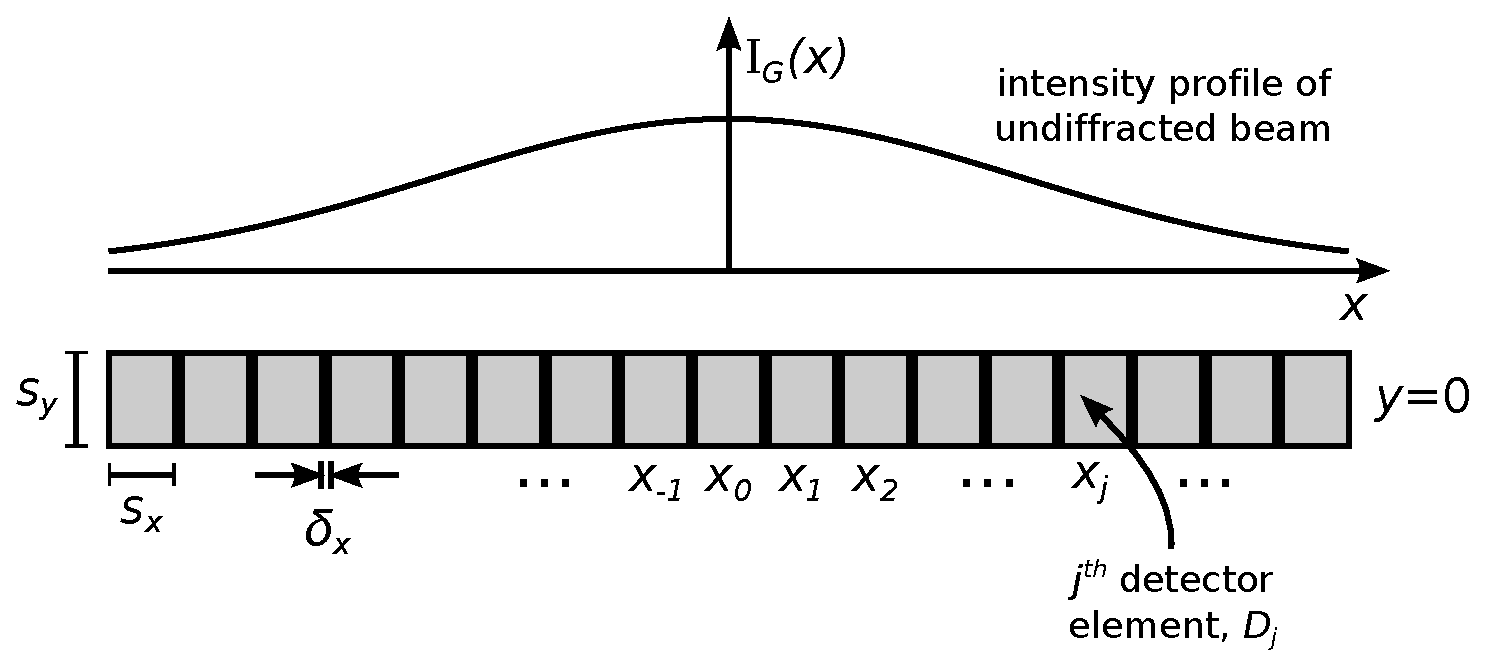
\includegraphics[width = \textwidth]{%
    Chapters/InterferometricMethods/figs/detector_array.eps}
  \caption[Finite sampling-volume effects in a detector array]{%
    The probe radiation and the reference beam
    are interfered on a detector array.
    The array consists of numerous detector elements,
    each of size $s_x \times s_y$ and with interelement spacing $\delta_x$.
    The undiffracted beam is centered on $x_0 = 0$ and $y = 0$, and
    its intensity profile varies only weakly over any given element.
    The finite size of each detector element tends to attenuate
    short wavelength components of the incident optical signal.
  }
  \label{fig:InterferometricMethods:detector_array}
\end{figure}

Homodyne detection results from using
a reference phase that is constant (or nearly constant) in time
such that the resulting intensity is
\begin{equation}
  \begin{aligned}
    I_{\text{hom}}(\vect{r}, t)
    =
    2 I_G(\vect{r})
    \bigl[%
      1
      &+
      \cos(\phi_R - \bar{\phi})
      \\
      &+
      \tilde{\phi}_0
      \sin(\phi_R - \bar{\phi}) \cos\xi
    \bigr]
  \end{aligned}
  \label{eq:InterferometricMethods:homodyne_intensity}
\end{equation}
Finite sampling-volume effects~\cite{bravenec_rsi95} dictate
the homodyne interferometer's wavenumber response~\cite{davis_rsi16}.
Assume that the probe radiation and the reference beam
are interfered on a detector array,
as shown in Fig.~\ref{fig:InterferometricMethods:detector_array}.
Let the $j$\ts{th} detector element $D_j$ be centered on $x_j$ and $y = 0$;
the total power $P_{j, \, \text{hom}}$ incident on this element is then
\begin{align}
  P_{j, \, \text{hom}}(t)
  &=
  \int_{D_j} I_{\text{hom}}(\vect{r}, t) dA
  \notag \\
  &\begin{aligned}
    \approx
    2 I_G(\vect{r_j}) s_y
    \int_{x_j - s_x / 2}^{x_j + s_x / 2}
    \bigl[%
      1
      &+
      \cos(\phi_R - \bar{\phi})
      \\
      &+
      \tilde{\phi}_0
      \sin(\phi_R - \bar{\phi}) \cos\xi
    \bigr] dx
  \end{aligned}
  \notag
\end{align}
where the weakly varying intensity profile $I_G(\vect{r})$
has been approximated as a constant
over the face of the detector element.
As the finite sampling-volume integral
will also be applied in other sections,
it is explicitly evaluated here for later reference
\begin{equation}
  \int_{x_j - s_x / 2}^{x_j + s_x / 2}
  \cos\xi dx
  =
  s_x \sinc\left( \frac{k}{k_c} \right) \cos\xi_j
  \label{eq:InterferometricMethods:finite_sampling_volume_integral}
\end{equation}
where
\begin{equation}
  \sinc(x) = \frac{\sin(\pi x)}{\pi x}
  \label{eq:InterferometricMethods:normalized_sinc}
\end{equation}
is the normalized sinc function,
\begin{equation}
  k_c = \frac{2 \pi M}{s_x}
  \label{eq:InterferometricMethods:finite_sampling_volume_cutoff}
\end{equation}
is the first zero (i.e.\ ``cutoff'') of the sinc function, and
\begin{equation}
  \xi_j = \frac{k x_j}{M} - \omega t
  \label{eq:InterferometricMethods:xi_j}
\end{equation}
Thus, the homodyne optical power becomes
\begin{align}
  \begin{aligned}
    P_{j, \, \text{hom}}(t)
    =
    2 I_G(\vect{r_j}) A
    &\bigl[%
      1
      +
      \cos(\phi_R - \bar{\phi})
      \\
      &+
      \tilde{\phi}_0
      \sin(\phi_R - \bar{\phi})
      \sinc(k / k_c)
      \cos\xi_j
    \bigr]
  \end{aligned}
  \label{eq:InterferometricMethods:homodyne_interferometer_total_power_per_element}
\end{align}
where $A = s_x s_y$ is the area of the detector element.

The typical engineering constraint of such a system
is the saturation intensity of the detector elements.
Beyond the linear saturation intensity $I_{\text{sat}}$,
the detector's response ceases to be a linear function
of the incident optical power.
For approximately uniform illumination,
the saturation threshold can be equivalently characterized
by a saturation power $P_{\text{sat}} \equiv I_{\text{sat}} A$.
To make an ``apples-to-apples'' comparison of different interference schemes,
it is useful to examine the ratio of the fluctuating power to $P_{\text{sat}}$.
To proceed, note that the homodyne optical power in
(\ref{eq:InterferometricMethods:homodyne_interferometer_total_power_per_element})
can be separated into equilibrium and fluctuating components as
$P_{j, \, \text{hom}}(t)
=
\bar{P}_{j, \, \text{hom}}
+
\tilde{P}_{j, \, \text{hom}}(t)$, where
\begin{align}
  \bar{P}_{j, \, \text{hom}}(t)
  &=
  2 I_G(\vect{r_j}) A
  [1 + \cos(\phi_R - \bar{\phi})]
  \\
  \tilde{P}_{j, \, \text{hom}}(t)
  &=
  2 I_G(\vect{r_j}) A
  \tilde{\phi}_0
  \sin(\phi_R - \bar{\phi})
  \sinc(k / k_c)
  \cos\xi_j
\end{align}
Then, because $\tilde{\phi}_0 \ll 1$
\begin{equation}
  P_{j, \, \text{hom}}
  \approx
  \bar{P}_{j, \, \text{hom}}
  \leq
  2 I_G(0) A [1 + \cos(\phi_R - \bar{\phi})]
  \notag
\end{equation}
where $I_G(0)$ is the peak intensity of the undiffracted Gaussian probe beam.
To obtain optimal performance, select $I_G(0)$ such that
\begin{equation}
  P_{\text{sat}}
  =
  2 I_G(0) A [1 + \cos(\phi_R - \bar{\phi})]
  \notag
\end{equation}
Then
\begin{equation}
  \frac{\tilde{P}_{j, \, \text{hom}}(t)}{P_{\text{sat}}}
  =
  \frac{I_G(\vect{r_j})}{I_G(0)}
  \cdot
  T_{\text{hom}}(k)
  \cdot
  \tilde{\phi}_0 \cos\xi_j
\end{equation}
where
\begin{equation}
  T_{\text{hom}}(k)
  \equiv
  \frac{\sin(\phi_R - \bar{\phi})}{1 + \cos(\phi_R - \bar{\phi})}
  \left[
    \sinc\left( \frac{k}{k_c} \right)
  \right]
  \label{eq:InterferometricMethods:homodyne_interferometer_wavenumber_transfer_function}
\end{equation}
is the homodyne interferometer's wavenumber transfer function.
That is, the homodyne interferometer
weights the phase-fluctuation images $\tilde{\phi}_0 \cos\xi_j$
by its transfer function $T_{\text{hom}}(k)$.
The prefactor $I_G(\vect{r_j}) / I_G(0)$
can (and should) be accounted for
if the beam profile is known.

Note that $T_{\text{hom}}(k)$ is a function
of the phase difference $\phi_R - \bar{\phi}$.
The homodyne interferometer operates at its peak sensitivity
when $|T_{\text{hom}}(k)|$ is maximal,
which occurs when $\phi_R - \bar{\phi} = \pi / 2 + m \pi$ for integer $m$.
For concreteness in the following discussion,
take $\phi_R - \bar{\phi} = \pi / 2$.
Physically, $\phi_R - \bar{\phi} = \pi / 2$
means that the reference beam is
out-of-phase with the undiffracted beam but
in-phase with the diffracted beams.
Note that interfering the diffracted beams with this in-phase reference beam
produces an intensity linear in $\tilde{\phi}_0$;
this should be contrasted with the situation
that produces the weak, quadratic intensity variation in
(\ref{eq:InterferometricMethods:imaged_field_intensity}).

Practically speaking, however,
it is very difficult to keep $\phi_R - \bar{\phi}$ fixed at $\pi / 2$.
First, a CO$_2$ beam passing through $\sim \SI{1}{\meter}$
of plasma with a density $n_e \sim \SI{e20}{\per\meter\cubed}$
will experience a bulk phase delay $\bar{\phi} \sim \pi$;
thus, for constant $\phi_R$, it will be impossible
to operate the interferometer at its peak sensitivity
($\phi_R - \bar{\phi} \approx \pi / 2$)
as the density evolves across the discharge.
Second, fusion experiments are often characterized
by large, pulsed electromagnets
whose vibrations can change the path lengths of the interferometer's arms.
A path-length change $\delta l$ produces
$\delta(\phi_R - \bar{\phi}) = k_0 \delta l$,
where $k_0$ is the wavenumber of the probe radiation.
For a $\SI{10.6}{\micro\meter}$ CO$_2$ probe beam,
a path-length variation $\sim \SI{2.5}{\micro\meter}$
is sufficient to produce $\delta(\phi_R - \bar{\phi}) \sim \pi / 2$,
pushing the homodyne interferometer from
its configuration of peak sensitivity into one of its nulls.
Even vacuum-pump vibrations can provide such a push!
On small fusion devices,
actively controlled mirrors have been used in an attempt
to account for the evolution of the equilibrium phase and
to cancel vibrational path-length changes,
minimizing excursions from $\phi_R - \bar{\phi} \approx \pi / 2$
\cite{nazikian_rsi87}, but
such an approach has not found application on larger
(and presumably more vibration-prone) fusion experiments.

In addition to its variable sensitivity,
the homodyne interferometer does \emph{not} make an absolute measurement
of the phase fluctuation amplitude $\tilde{\phi}_0$
\cite[Sec.~4.2.2]{hutchinson_diagnostics}.
For example, vibration-induced misalignment or
power fluctuations at the beam source
can alter the intensity $I_G(\vect{r_j})$.
As a result, there are three potentially dynamic quantities:
$\{\phi_R - \bar{\phi}, \tilde{\phi}_0, I_G(\vect{r_j})\}$, but
there are only two measured quantities:
the equilibrium and fluctuating homodyne powers.
Thus, it is generally impossible to distinguish
whether changes in the amplitude of the fluctuating power
are attributable to real changes in $\tilde{\phi}_0$ or
are simply an artifact of the system alignment or radiation source.


\subsection{Heterodyne detection}
\graffito{\textcolor{blue}{Qualitative figure of baseband vs IF}}
To avoid the above-mentioned challenges of homodyne interferometry,
the reference phase can be linearly ramped in time
as $\phi_R = \Delta \omega_0 t$ such that
the intensity becomes
\begin{equation}
  \begin{aligned}
    I_{\text{het}}(\vect{r}, t)
    =
    2 I_G(\vect{r})
    \bigl[%
      1
      &+
      \cos(\Delta \omega_0 t - \bar{\phi})
      \\
      &+
      \tilde{\phi}_0
      \sin(\Delta \omega_0 t - \bar{\phi}) \cos\xi
    \bigr]
  \end{aligned}
  \label{eq:InterferometricMethods:heterodyne_intensity}
\end{equation}
This approach is known as heterodyne interferometry,
as the desired baseband phase information is shifted
to an intermediate frequency $\Delta \omega_0$
satisfying $(d\phi/dt)_{\text{max}} \ll \Delta \omega_0 \ll \omega_0$.
\graffito{\textcolor{red}{This will be discussed more in Ch.~3}}
Practically, the $\phi_R$ ramp is accomplished by modestly Doppler shifting
the reference beam relative to the plasma beam.

As is the case for homodyne detection,
finite sampling-volume effects~\cite{bravenec_rsi95} dictate
the heterodyne interferometer's wavenumber response~\cite{davis_rsi16}.
The following discussion closely parallels that
of the homodyne interferometer in
Section~\ref{sec:InterferometricMethods:interferometry:homodyne}, and
readers are encouraged to review that section if needed and
to compare and contrast homodyne and heterodyne detection.
Assume that the probe radiation and the reference beam
are interfered on a detector array,
as shown in Fig.~\ref{fig:InterferometricMethods:detector_array}.
Let the $j$\ts{th} detector element $D_j$ be centered on $x_j$ and $y = 0$;
the total power $P_{j, \, \text{het}}$ incident on this element is then
\begin{align}
  P_{j, \, \text{het}}(t)
  &=
  \int_{D_j} I_{\text{het}}(\vect{r}, t) dA
  \notag \\
  &\begin{aligned}
    \approx
    2 I_G(\vect{r_j}) s_y
    \int_{x_j - s_x / 2}^{x_j + s_x / 2}
    \bigl[%
      1
      &+
      \cos(\Delta \omega_0 t - \bar{\phi})
      \\
      &+
      \tilde{\phi}_0
      \sin(\Delta \omega_0 t - \bar{\phi}) \cos\xi
    \bigr] dx
  \end{aligned}
  \notag \\
  &\begin{aligned}
    =
    2 I_G(\vect{r_j}) &A
    \bigl[%
      1
      +
      \cos(\Delta \omega_0 t - \bar{\phi})
      \\
      &+
      \tilde{\phi}_0
      \sin(\Delta \omega_0 t - \bar{\phi})
      \sinc(k / k_c)
      \cos\xi_j
    \bigr]
  \end{aligned}
  \label{eq:InterferometricMethods:heterodyne_interferometer_total_power_per_element}
\end{align}
where the weakly varying intensity profile $I_G(\vect{r})$
has been approximated as a constant
over the face of the detector element, and
the finite sampling-volume integral in
(\ref{eq:InterferometricMethods:finite_sampling_volume_integral})
has been referenced.
Note that the dominant Fourier components of $P_{j, \, \text{het}}$
sit at the intermediate frequency $\pm \Delta \omega_0$ but that
the phase-fluctuation term $\sin(\Delta \omega_0 t - \bar{\phi}) \cos\xi_j$
produce sidebands at $\pm (\Delta \omega_0 \pm \omega)$.

The heterodyne interference signal must be demodulated
in order to retrieve the baseband phase-fluctuation information.
\graffito{\textcolor{red}{More on demodulation hardware in Ch.~3}}
Practically speaking, dedicated analog or digital electronics
are used to demodulate the heterodyne signal;
however, for the pedagogical purposes of this section,
it is sufficient to consider the ``equivalent optical powers''
corresponding to the demodulated signals.
The so-called in-phase ($I$) and quadrature ($Q$) signals
are obtained by mixing $P_{j, \, \text{het}}$ with
$\cos( \Delta \omega_0 t)$ and $\sin( \Delta \omega_0 t)$, respectively, and
low-pass filtering the resulting signals;
here, low-pass filtering is implemented
by averaging over a cycle of the intermediate frequency.
Thus, the equivalent $I$ and $Q$ optical powers are defined as
\begin{align}
  P_{j, I}(t)
  &\equiv
  \langle
    \cos (\Delta \omega_0 t) \cdot P_{j, \, \text{het}}(t)
  \rangle_{\Delta \omega_0}
  \\
  P_{j, Q}(t)
  &\equiv
  \langle
    \sin (\Delta \omega_0 t) \cdot P_{j, \, \text{het}}(t)
  \rangle_{\Delta \omega_0}
\end{align}
where $\langle q \rangle_{\Delta \omega_0}$ denotes
the average of quantity $q$ over an intermediate-frequency cycle as
\begin{equation}
  \langle q \rangle_{\Delta \omega_0}
  \equiv
  \frac{\Delta \omega_0}{2 \pi}
  \int_{0}^{\Delta \omega_0 / 2 \pi}
  q(t) dt
  \label{eq:InterferometricMethods:intermediate_frequency_cycle_average}
\end{equation}
Note that $P_{j,I}$ and $P_{j,Q}$ can be conveniently combined as
\begin{align}
  P_{j,I} + i \cdot P_{j,Q}
  &=
  \langle
    e^{i \Delta \omega_0 t} \cdot P_{j, \, \text{het}}(t)
  \rangle_{\Delta \omega_0}
  \notag \\
  &=
  I_G(\vect{r_j}) A
  e^{i \bar{\phi}}
  \left[%
    1
    +
    i \tilde{\phi}_0 \sinc(k / k_c) \cos\xi_j
  \right]
  \label{eq:InterferometricMethods:heterodyne_interferometer_I_and_Q_power_per_element}
\end{align}

In contrast to the homodyne interferometer,
the heterodyne interferometer makes an absolute measurement
of the phase-fluctuation amplitude $\tilde{\phi}_0$.
To see this, note that $P_{j,I}$ and $P_{j,Q}$ in
(\ref{eq:InterferometricMethods:homodyne_interferometer_total_power_per_element})
can be separated into equilibrium and fluctuating components as
\begin{align}
  \bar{P}_{j,I}(t)
  &=
  I_G(\vect{r_j}) A \cos\bar{\phi}
  \\
  \bar{P}_{j,Q}(t)
  &=
  I_G(\vect{r_j}) A \sin\bar{\phi}
  \\
  \tilde{P}_{j,I}(t)
  &=
  -I_G(\vect{r_j}) A
  \tilde{\phi}_0
  \sin\bar{\phi} \,
  \sinc(k / k_c)
  \cos\xi_j
  \\
  \tilde{P}_{j,Q}(t)
  &=
  I_G(\vect{r_j}) A
  \tilde{\phi}_0
  \cos\bar{\phi} \,
  \sinc(k / k_c)
  \cos\xi_j
\end{align}
As is the case for the homodyne interferometer,
there are three potentially dynamic quantities:
$\{\bar{\phi}, \tilde{\phi}_0, I_G(\vect{r_j})\}$;
however, in contrast to the homodyne interferometer,
there are now \emph{four} measured quantities:
$\{\bar{P}_{j,I}, \bar{P}_{j,Q}, \tilde{P}_{j,I}, \tilde{P}_{j,Q}\}$.
Therefore, the number of measured quantities
is sufficient to unambiguously determine
$\{\bar{\phi}, \tilde{\phi}_0, I_G(\vect{r_j})\}$
in absolute units.

Finally, it is useful to characterize
the heterodyne interferometer's performance
relative to the saturation limits of a given detector.
Because $\tilde{\phi}_0 \ll 1$,
(\ref{eq:InterferometricMethods:heterodyne_interferometer_total_power_per_element})
can be approximated as
\begin{align}
  P_{j, \, \text{het}}
  &\approx
  2 I_G(\vect{r_j}) A [1 + \cos(\Delta \omega_0 t - \bar{\phi})]
  \notag \\
  &\leq
  4 I_G(0) A
  \notag
\end{align}
where $I_G(0)$ is the peak intensity of the undiffracted Gaussian probe beam.
To obtain optimal performance, select $I_G(0)$ such that
\begin{equation}
  P_{\text{sat}}
  =
  4 I_G(0) A
  \notag
\end{equation}
Further, define the total fluctuating power
in the demodulated signals to be
\begin{align}
  \tilde{P}_{j, IQ}(t)
  &\equiv
  \left\{%
    [\tilde{P}_{j,I}(t)]^2
    +
    [\tilde{P}_{j,Q}(t)]^2
  \right\}^{1/2}
  \notag \\
  &=
  I_G(\vect{r_j}) A
  \tilde{\phi}_0
  \sinc(k / k_c)
  \cos\xi_j
\end{align}
such that
\begin{equation}
  \frac{\tilde{P}_{j, IQ}(t)}{P_{\text{sat}}}
  =
  \frac{I_G(\vect{r_j})}{I_G(0)}
  \cdot
  T_{\text{het}}(k)
  \cdot
  \tilde{\phi}_0
  \cos\xi_j
  \label{}
\end{equation}
where
\begin{equation}
  T_{\text{het}}(k)
  \equiv
  \frac{1}{4}
  \sinc\left( \frac{k}{k_c} \right)
  \label{eq:InterferometricMethods:heterodyne_interferometer_wavenumber_transfer_function}
\end{equation}
is the heterodyne interferometer's wavenumber transfer function.
That is, the heterodyne interferometer
weights the phase-fluctuation images $\tilde{\phi}_0 \cos\xi_j$
by its transfer function $T_{\text{het}}(k)$.
The prefactor $I_G(\vect{r_j}) / I_G(0)$
can (and should) be accounted for
if the beam profile is known.

In contrast to the homodyne interferometer,
the heterodyne interferometer's wavenumber transfer function
is \emph{not} a function of $\phi_R - \bar{\phi}$.
Thus, the heterodyne interferometer always operates at its peak sensitivity,
regardless of the bulk plasma phase or path-length vibrations.
Robust sensitivity comes at a cost, however.
Note that
\begin{equation}
  \frac{T_{\text{het}}(k)}{T_{\text{hom}}(k)}
  =
  \frac{1}{4}
  \quad
  \text{for homodyne operation at $\phi_R - \bar{\phi} = \pi / 2$}
  \notag
\end{equation}
Thus, for a given detector,
a heterodyne interferometer will be four times \emph{less} sensitive
than a homodyne interferometer operated in its optimal configuration
($\phi_R - \bar{\phi} = \pi / 2$).
This factor of four has two physical origins.
First, the detector of a homodyne interferometer
with a fixed $\phi_R - \bar{\phi} = \pi / 2$
only sees small fluctuations about a DC offset, while
the detector of a heterodyne interferometer
sees the full sinusoidal waveform of the intermediate frequency;
to ensure the detector is always within its saturation limits,
the heterodyne interferometer must necessarily be operated with
a mean intensity at the detector
that is a factor of two lower than that for the homodyne interferometer.
Second, the mixing process
that is used to demodulate the heterodyne interference signal
results in a loss of half of the signal power.


\section{Phase contrast imaging (PCI)}
\label{sec:InterferometricMethods:pci}
As discussed in
Section~\ref{sec:InterferometricMethods:imaging:need_for_reference_beam},
imaging the probe radiation on a square-law detector
produces a very weak response
because the undiffracted and diffracted beams
are $\pi / 2$ out of phase with each other.
To produce a measurable response, a traditional interferometer
interferes the imaged radiation with an external reference beam.
If the phase of the undiffracted beam could be manipulated, though,
the external reference beam would no longer be needed.
This is the approach employed in phase contrast imaging (PCI).


\subsection{Reference-beam generation with a phase plate}
PCI uses an optical element known as a \emph{phase plate}
to delay the undiffracted beam by $\pi / 2$
relative to the diffracted beams.
The phase plate is typically a reflective optical element
with a groove that is precisely fabricated
to have a depth of $\lambda_0 / 8$;
the undiffracted beam reflects off of this groove, and
the corresponding $\lambda_0 / 4$-increase in path length
phase delays the undiffracted beam by $\pi / 2$
relative to the diffracted beams,
which reflect off of the non-grooved portions of the phase plate.
To boost the relative size of the fluctuating signal,
the phase groove typically reflects only a fraction $\eta < 1$
of the incident undiffracted beam power, while
the non-grooved portions of the phase plate
reflect all of the diffracted beam power.
Thus, by the action of the phase plate,
the electric field in the PCI image plane becomes
\begin{equation}
  E_{\text{PCI}}(\vect{r}, t)
  =
  i E_G(\vect{r}, t) e^{i \bar{\phi}}
  \left[%
    \sqrt{\eta} + \tilde{\phi}_0 \cos\xi
  \right]
  \label{eq:InterferometricMethods:pci_imaged_field}
\end{equation}
and, to first order in $\tilde{\phi}_0$, the corresponding intensity is
\begin{equation}
  I_{\text{PCI}}(\vect{r}, t)
  =
  I_G(\vect{r})
  \left[%
    \eta
    +
    2 \sqrt{\eta} \tilde{\phi}_0 \cos\xi
  \right]
  \label{eq:InterferometricMethods:pci_intensity}
\end{equation}
where $E_G(\vect{r})$ and $I_G(\vect{r})$ would be
the field and intensity profiles
of the undiffracted Gaussian beam on the detector
in the \emph{absence} of the phase plate;
$I_G(\vect{r})$ is defined in
(\ref{eq:InterferometricMethods:Gaussian_beam_intensity}).
Equations
(\ref{eq:InterferometricMethods:pci_imaged_field}) and
(\ref{eq:InterferometricMethods:pci_intensity})
should be contrasted with their corresponding equations
in the absence of the phase plate:
(\ref{eq:InterferometricMethods:imaged_total_field_weak_coupling}) and
(\ref{eq:InterferometricMethods:imaged_field_intensity}), respectively.
Thus, the phase plate converts the undiffracted probe beam
into an effective reference beam for the diffracted beams.


\subsection{Focal-plane separation of diffracted beams}
Implicit in the use of the phase plate
is that the undiffracted and diffracted beams
are well-separated in space
such that the phase groove only affects the undiffracted beam.
The 1\ts{st}-order diffracted beams are angularly separated
from the undiffracted beam by $\theta = k / k_0$.
\graffito{\textcolor{red}{Sufficiently large: $k w_0 \gtrsim 2$?}}
Provided that $\theta$ is sufficiently large,
the diffracted and undiffracted beams
will be spatially separated in the far-field
($z \gg z_R$, with $z_R$ being the Rayleigh length of the in-vessel beam);
however, $z \gg z_R$ is not easily accessed in typical lab settings.
Fortunately, the far-field diffraction pattern
can be equivalently accessed in the focal plane
\graffito{\textcolor{red}{Chapter???}}
of a focusing optic~\cite{born_and_wolf}.

The focal-plane location, beam size, and beam separation
can be easily determined.
Let the Gaussian probe beam have
an in-vessel 1/e $E$ waist radius of $w_0$,
and place a focusing optic of focal length $f$
a distance $s$ downstream from the in-vessel beam waist.
Then, the waist of the focused beam
will be located a distance $s'$ downstream of the focusing optic
and will have 1/e $E$ radius $w_0'$ given as
\begin{align}
  s' &= f \left( 1 + \frac{s - f}{z_R} \right)
  \label{eq:InterferometricMethods:focal_plane_location_general}
  \\
  w_0' &= \frac{w_0 |f|}{\left[ (s - f)^2 + z_R^2 \right]^{1/2}}
  \label{eq:InterferometricMethods:focal_plane_waist_general}
\end{align}
where $z_R$ is the in-vessel Rayleigh length~\cite{self83}.
When $|s - f| \ll z_R$, as is typical for PCI,
(\ref{eq:InterferometricMethods:focal_plane_location_general}) and
(\ref{eq:InterferometricMethods:focal_plane_waist_rayleigh}) become
\graffito{\textcolor{red}{%
  Simple optics gives correct $s'$, but
  Gaussian beam physics needed for $w_0'$}
}%
\begin{align}
  s' &\approx f
  \label{eq:InterferometricMethods:focal_plane_location_rayleigh}
  \\
  w_0' &\approx \frac{2 |f|}{k_0 w_0}
  \label{eq:InterferometricMethods:focal_plane_waist_rayleigh}
\end{align}
The spatial separation $\Delta$
of the diffracted beam from the undiffracted beam
in the focal lane is found through the corresponding ray matrices
\begin{align}
  \begin{pmatrix}
    \Delta
    \\
    \theta_{pp}
  \end{pmatrix}
  &=
  \begin{pmatrix}
    1 & s'
    \\
    0 & 1
  \end{pmatrix}
  \begin{pmatrix}
    1      & 0
    \\
    -1 / f & 1
  \end{pmatrix}
  \begin{pmatrix}
    1 & s
    \\
    0 & 1
  \end{pmatrix}
  \begin{pmatrix}
    0
    \\
    \theta
  \end{pmatrix}
\end{align}
which simplifies to
\begin{equation}
  \Delta
  =
  \frac{k |f|}{k_0}
  \label{eq:InterferometricMethods:phase_plate_beam_separation}
\end{equation}


\subsection{Low-$k$ cutoff of phase plate}
Now, let the phase plate groove have a width $d$.
Finite PCI response requires that (most of) the diffracted beams
fall outside of the phase groove (e.g.\ $\Delta \geq d / 2$
such that at least half of the scattered beam
falls outside of the phase groove).
Application of (\ref{eq:InterferometricMethods:phase_plate_beam_separation})
then shows that there will be finite PCI response
for $k \geq k_g$ where
\begin{equation}
  k_g \equiv \frac{k_0 d}{2 f}
  \label{eq:InterferometricMethods:pci_kmin_engineering}
\end{equation}
Here, the subscript $g$ is in reference
to the \emph{groove} of the phase plate.
Further, the scattering process is usually very weak.
To avoid saturating the detector with the signal from the unscattered beam,
the unscattered beam should fall wholly within the phase groove
($2 w_0' \leq d$), which usually has a reflectivity $\eta \ll 1$.
Application of (\ref{eq:InterferometricMethods:focal_plane_waist_rayleigh})
then yields a constraint on the phase groove width
\begin{equation}
  d \geq \frac{4 |f|}{k_0 w_0}
  \label{eq:InterferometricMethods:phase_groove_constraint}
\end{equation}
and inserting (\ref{eq:InterferometricMethods:phase_groove_constraint}) into
(\ref{eq:InterferometricMethods:pci_kmin_engineering}) yields
\begin{equation}
  k_g \geq \frac{2}{w_0}
  \label{eq:pci_kmin_physics}
\end{equation}
\graffito{\textcolor{red}{%
  Note that this is the same limit as for true far-field spatial separation
  (i.e.\ when not using focal-plane spatial separation)}
}%
That is, PCI's low-$k$ cutoff
is ultimately constrained by the in-vessel beam size $w_0$,
with diffraction being the constraining physical mechanism.


\subsection{High-$k$ cutoff of phase plate}
Let the phase plate have a diameter $D$.
Detection of the diffracted radiation
requires that (most of) the diffracted beam reflect
from the face of the phase plate
(e.g.\ $\Delta \leq D / 2$).
Application of (\ref{eq:InterferometricMethods:phase_plate_beam_separation})
then shows that there will be finite PCI response for $k \leq k_D$ where
\begin{equation}
  k_D \equiv \frac{k_0 D}{2 f}
  \label{eq:InterferometricMethods:pci_kmax_engineering}
\end{equation}


\subsection{Wavenumber transfer function}
\label{sec:InterferometricMethods:pci:wavenumber_response}
The action of the phase plate is easily described in wavenumber space
via the transfer function
\begin{equation}
  \begin{aligned}
    T_{\text{pp}}(k_x)
    &=
    i \sqrt{\eta} \, H(k_g - |k_x|)
    \\
    &\quad +
    H(|k_x| - k_g)
    H(k_D - |k_x|)
  \end{aligned}
  \label{eq:InterferometricMethods:phase_plate_transfer_function}
\end{equation}
where $H(x)$ is the Heaviside step function defined as
\begin{equation}
  H(x)
  =
  \begin{cases}
    0, \quad &x < 0 \\
    1, \quad &x \geq 0
  \end{cases}
  \label{eq:InterferometricMethods:Heaviside_step_function}
\end{equation}
$k_g$ is given by
(\ref{eq:InterferometricMethods:pci_kmin_engineering}), and
$k_D$ is given by
(\ref{eq:InterferometricMethods:pci_kmax_engineering}).


\bibliographystyle{plainurl}
\bibliography{references}
